\section{Results and Discussion}

All the plots in this sections are made by the authors using matplotlib\cite{matplotlib}. We would like to acknowledge NumPy\cite{numpy} and SciPy\cite{scipy} for providing the necessary tools to vizualize, preprocess and derive meaningful insights from the simulations.

\subsection{Normal incidence}
In this section, we will discuss the results of the simulations for normal incidence. A number of simulations are performed to study the different laser and plasma parameters on the generated HHG and the plasma oscillations. We will first start by discussing how overdense and underdense plasma behaves in presence of relativistic and non-relativistic laser pulse.

\subsubsection{Preliminary Analysis}

\begin{figure}[H]
    \centering
    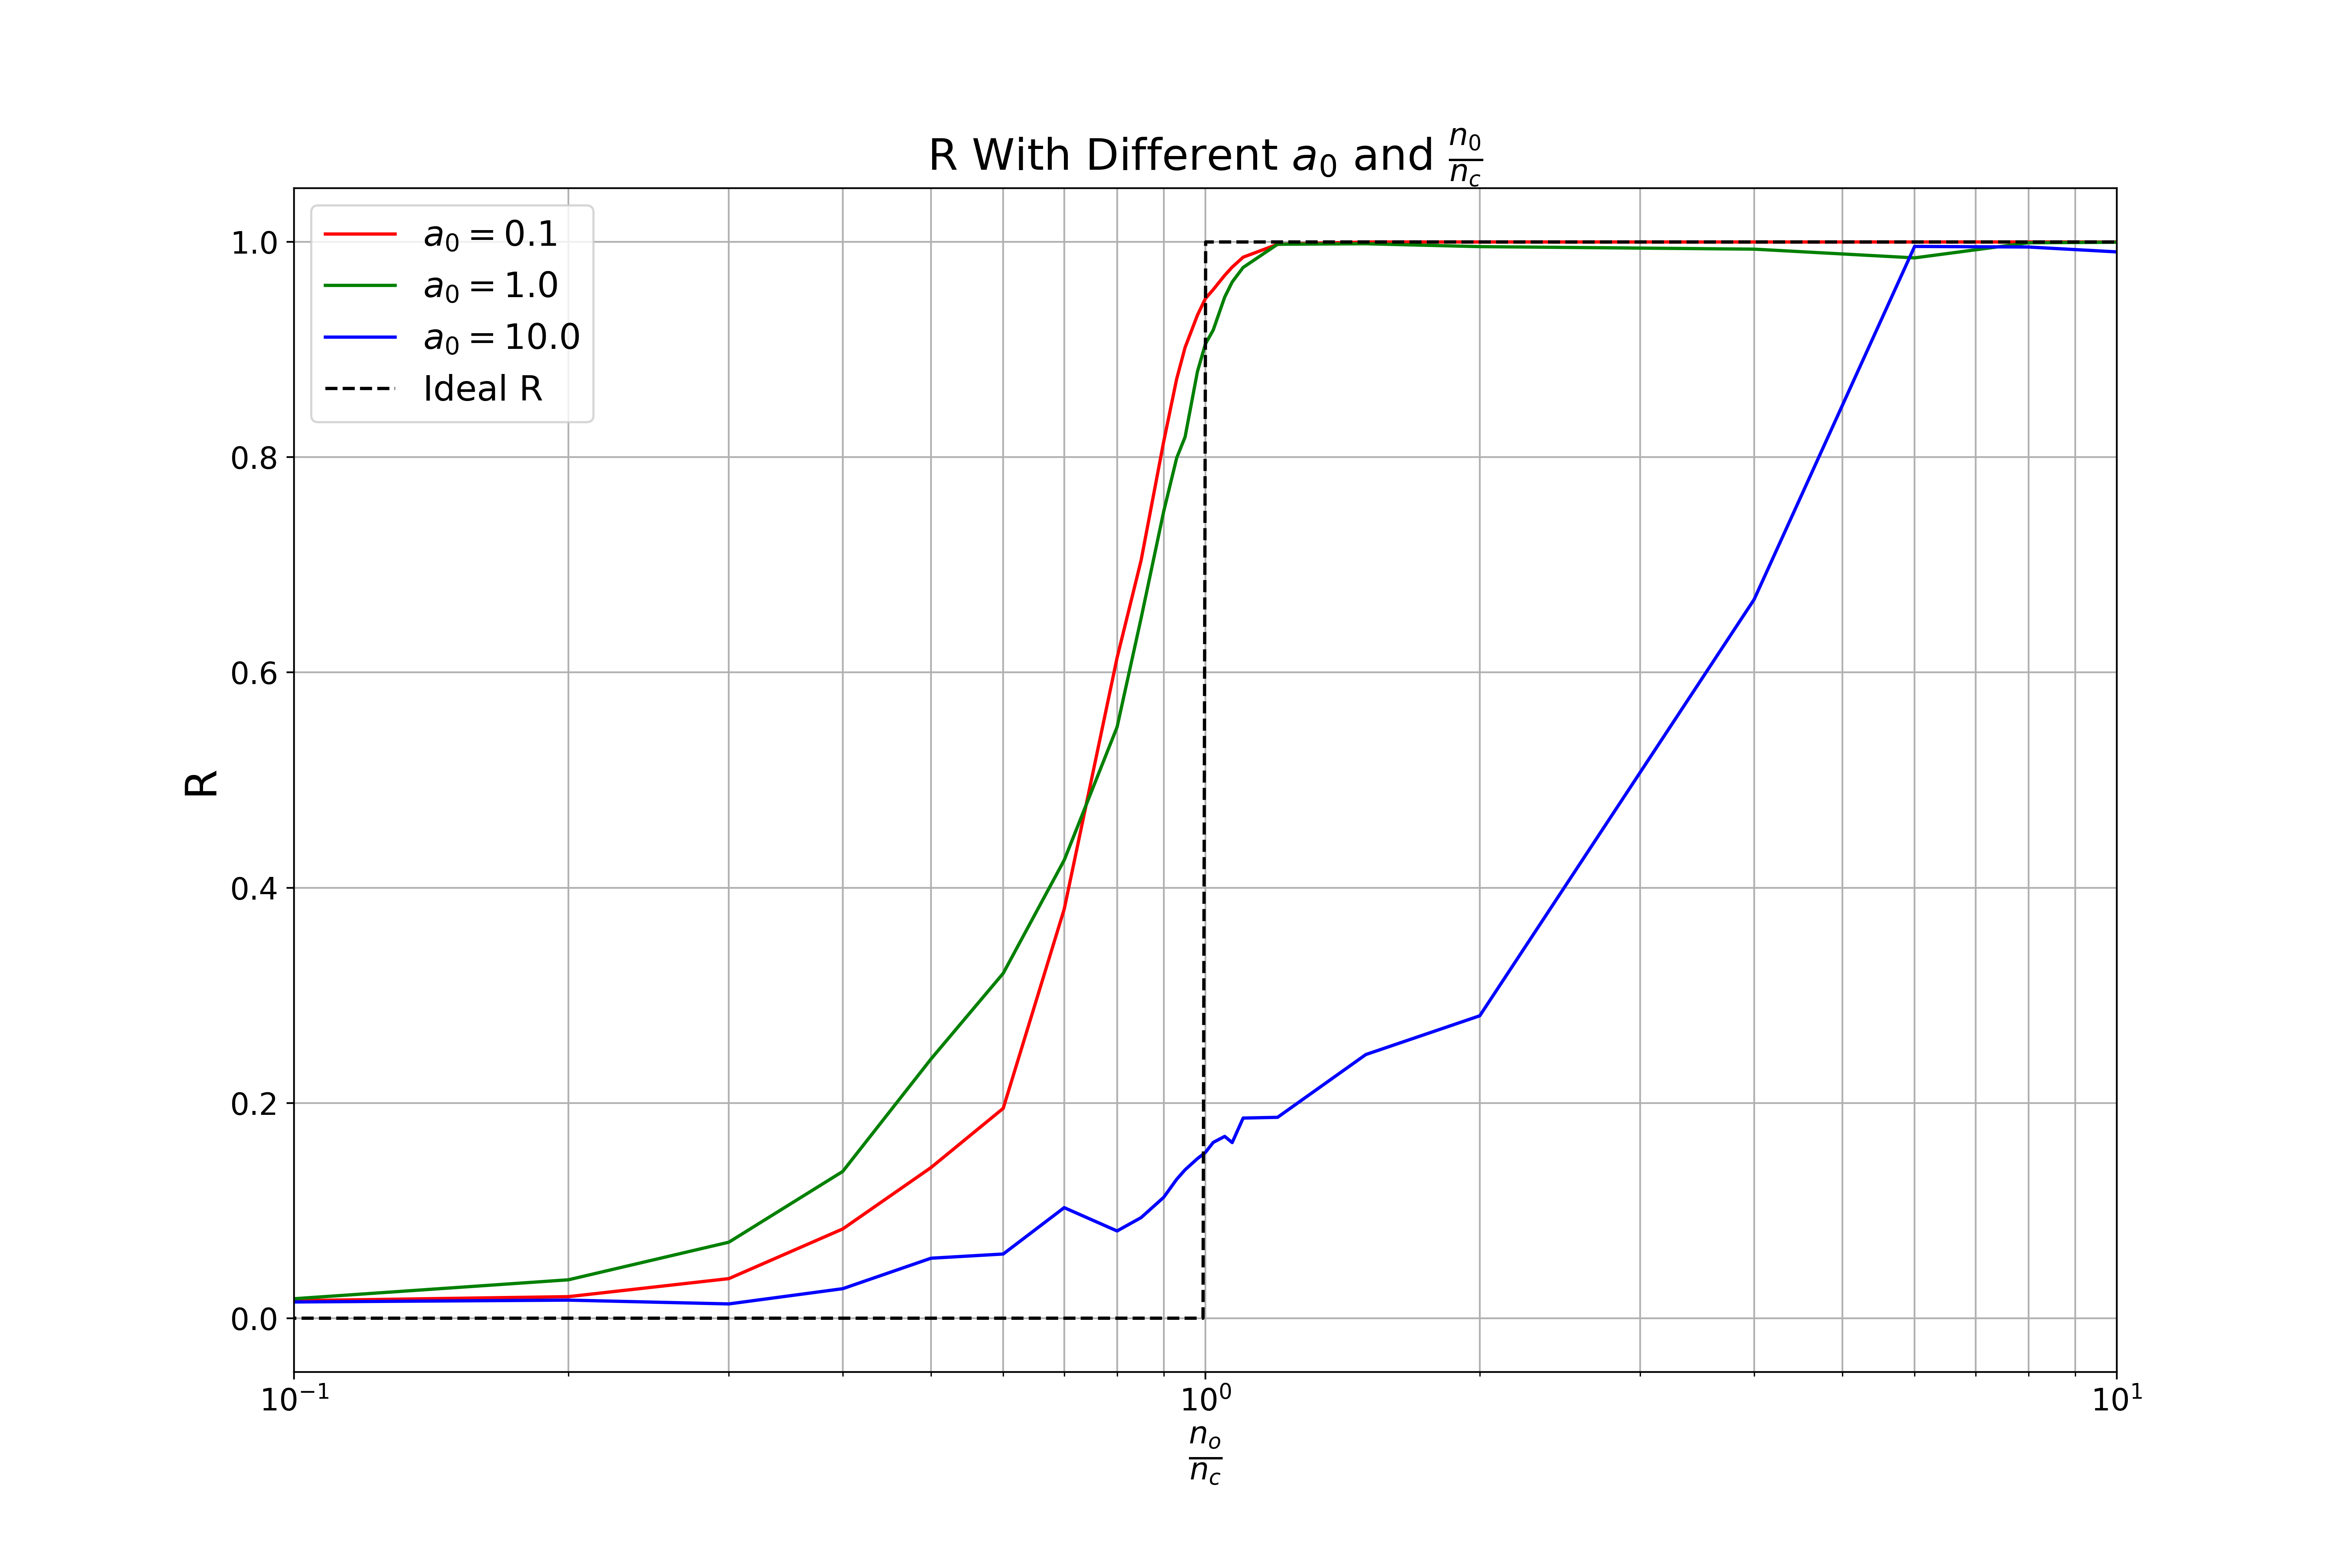
\includegraphics[width=0.75\textwidth]{reflectance.png}
    \caption{Plot of reflectance (see \ref{eq:reflectance}) with different ratio of $n_c$ and $n_0$ and vector potential $a_0$. Black dotted line represents the ideal behavior.}
    \label{fig:reflectance}
\end{figure}

The goal is to study the transmittence and reflectance of the laser pulse in underdense and overdense plasma for relativistic and non-relativistic case. For this, we define a term calling it the \textit{reflectance} as:

\begin{equation}
    \label{eq:reflectance}
    R = \frac{{E_{b}^2}-{E_{a}^2}}{{E_{b}^2}}
\end{equation}

where $E_{b}$ is the sum of y component of the electric field at a node before the plasma starts and $E_{a}$ is the sum of y component of the electric field at a node where plasma just ends. This way, the above relation gives a indication of the ratio of the intensity passing through the plasma to the intensity getting reflected.

The ideal curve for the interaction of laser pulse with underdense and overdense plasma is also shown in the figure with black dotted line. Ideally, when the ratio $r = \frac{n_0}{n_c}$ becomes 1, the reflectance also becomes 1. However, when the laser becomes relativistic for $a_0 \ge 1$, the particles inside plasma starts to oscillate with relativistic velocity, gaining mass. This results in change in the plasma frequency and hence the laser does not get reflected even for density greater than the critical density corresponding to the non-relativistic case. So, there is a shift in the critical density due to relativistic laser pulse.

Next, the plot of these oscillation of plasma surface with time is also shown for different values of vector potential (Figure \ref{fig:density_oscillations}). The plasma density is taken to be critical density, i.e., $r=1$. The laser pulse, after interacting with electrons, makes them oscillate. If the pulse becomes relativistic, the oscillations becomes strong and hence the plasma surface oscillates with relativistic velocity.



\begin{figure}[H]
    \centering
    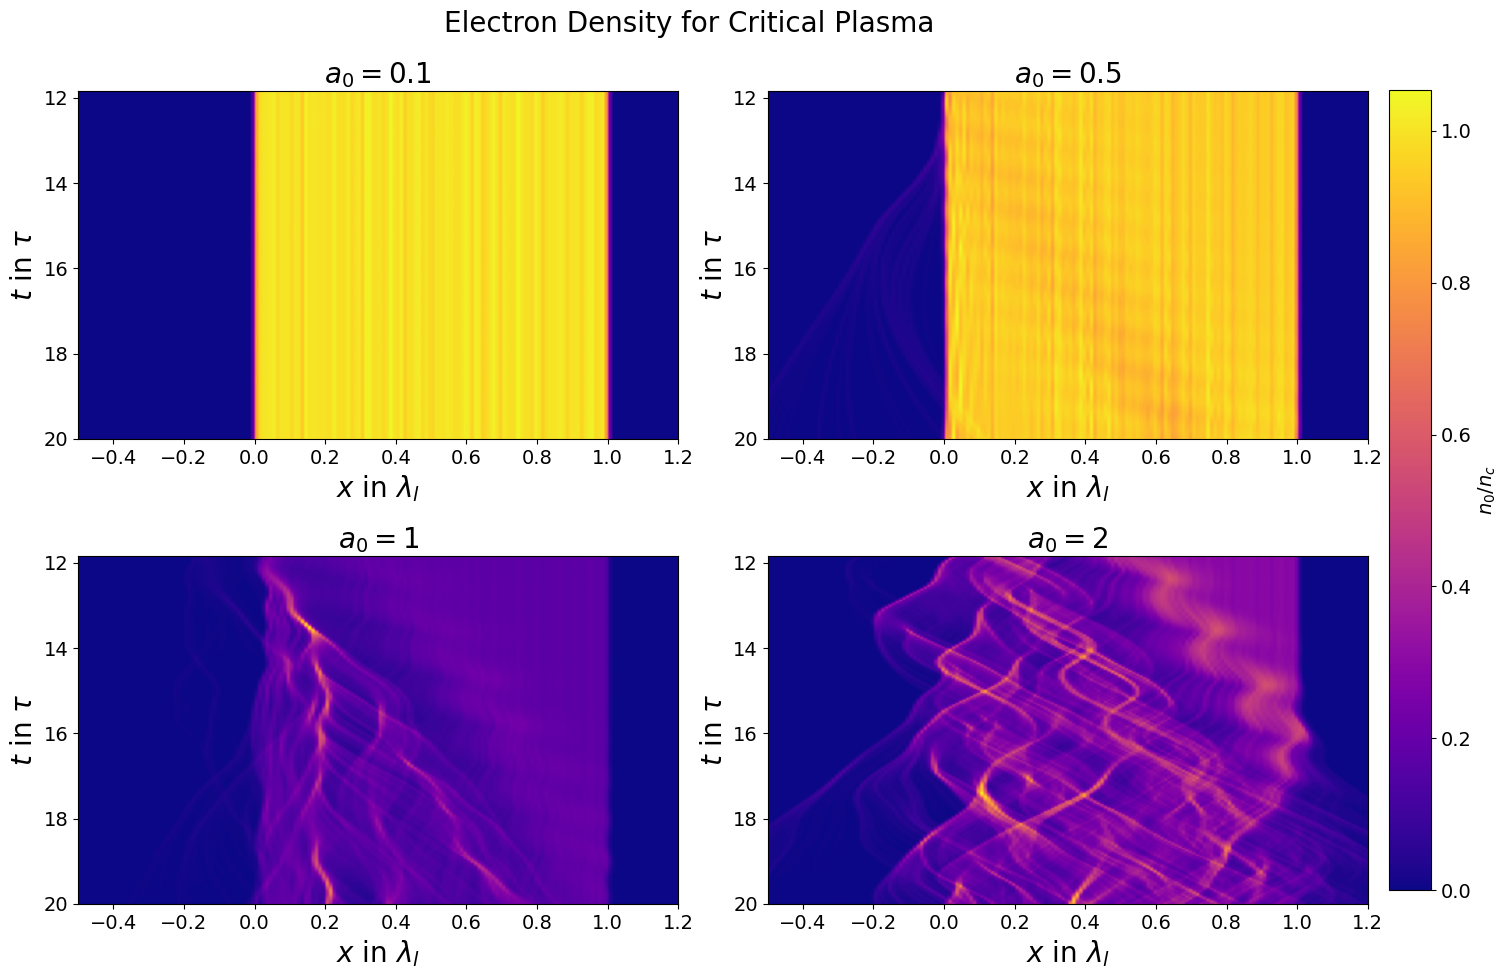
\includegraphics[width=0.95\textwidth]{density_oscillations.png}
    \caption{The effect of relativistic laser pulse on the plasma density oscillations. For $a_0=0.1$, the oscillation is very weak. As $a_0$ increases, the oscillation becomes stronger.}
    \label{fig:density_oscillations}
\end{figure}

\subsubsection{Effects On Generated HHG}
This section shows results which were obtained by varying the laser and plasma parameters.

\subsubsubsection{Effect of Plasma Density}
No significant effect of plasma density on generation of high harmonics is observed. However, a resonace is observed at plasma density of $4n_c$ giving more harmonics at that density (See figure \ref{fig:density}). This resonace is because the plasma frequency is equal to the frequency of the driving pondermotive force. (Since $F\propto (1-\cos{2\omega t})$)

\begin{figure}[H]
    \centering
    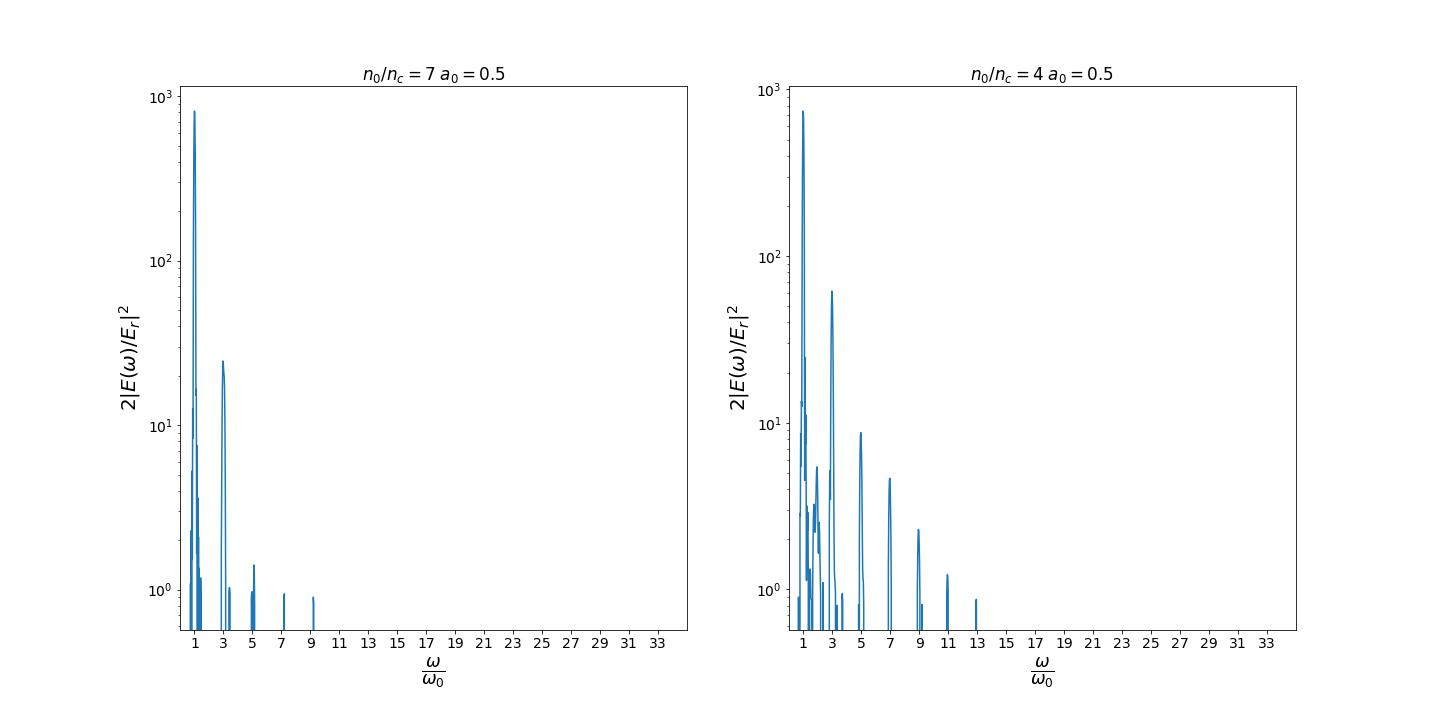
\includegraphics[width=1\textwidth]{density.jpg}
    \caption{Resonance at $n = 4n_c$}
    \label{fig:density}
\end{figure}

\subsubsubsection{Effect of Pre-Plasma}

Often, the laser is not able to interact with the main plasma target isolately. The reason behind this is that laser has prepulses which creates a pre-plasma. We wanted to study the effect of this pre-plasma on the generated HHG. For this, we created a \textit{ramp} of plasma of different length before the main plasma and studied its effect. The result was that if a pre-plasma is created before the laser starts interacting with the main plasma target, the efficiency of the generated HHG are decreased as the amplitude of the HHG are suppressed. See figure \ref{fig:ramp}.

\begin{figure}[H]
    \centering
    \subfloat[\centering The spectrum of the reflected field with and without a pre-plasma. A suppression in the HHG amplitude is observed for case with pre-plasma.]{{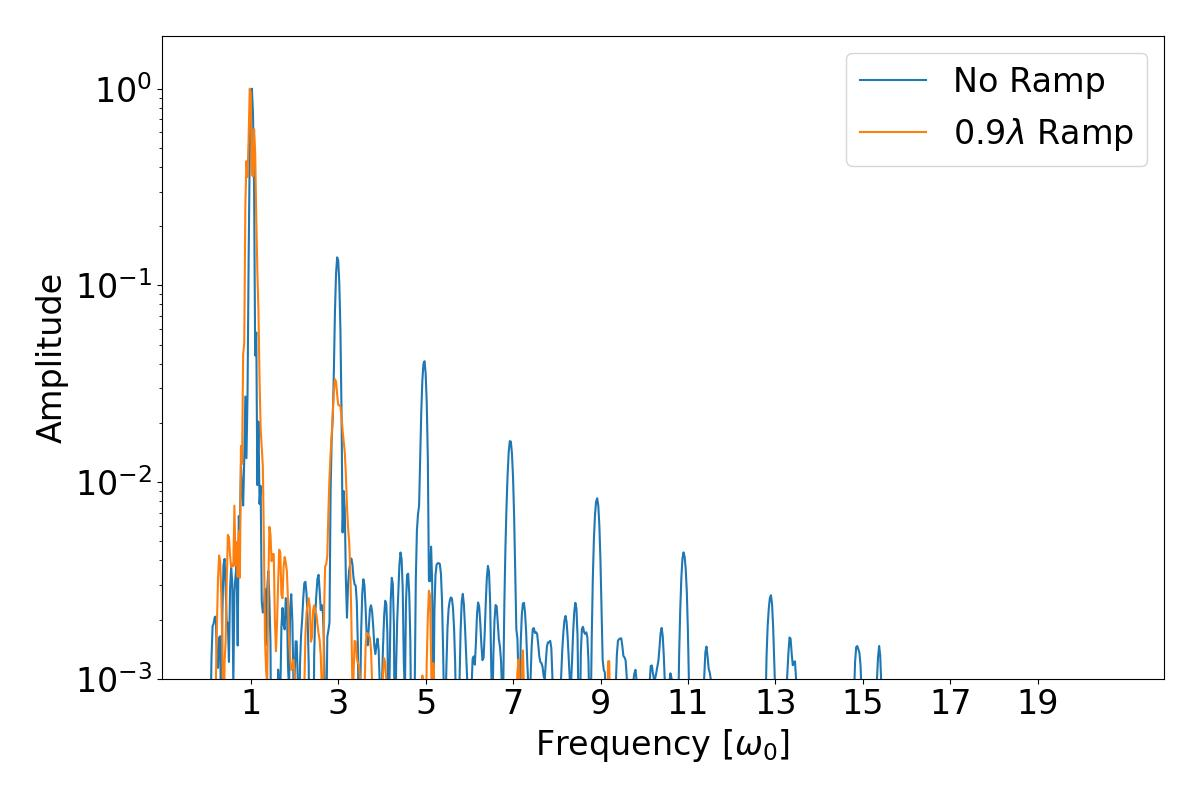
\includegraphics[width=0.47\textwidth, height=7cm]{ramp.jpg}}}%
    \quad
    \subfloat[\centering The peak of different harmonics for different ramp. The figure shows that as the ramp length increases, the amplitudes of the harmonics decreases.]{{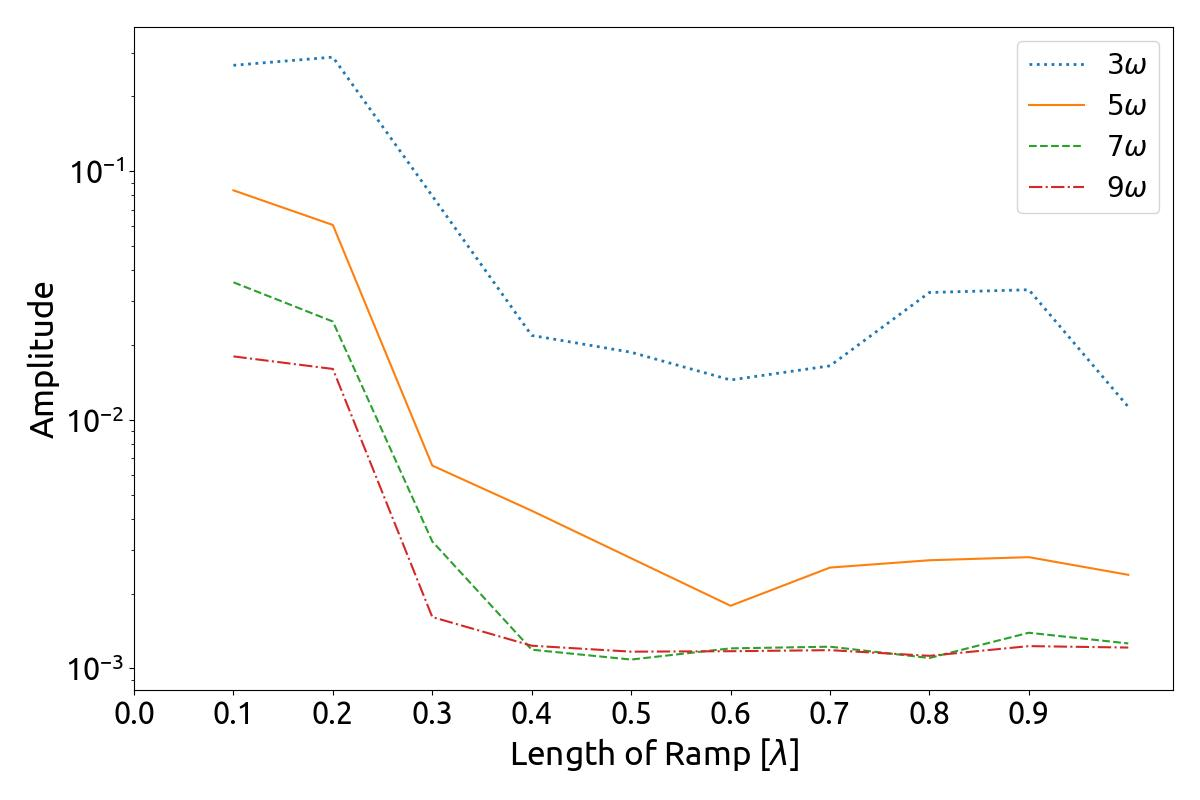
\includegraphics[width=0.47\textwidth, height=7cm]{ramp_7600.jpg}}}%
    \caption{Effect of Pre-Plasma. Other parameters are $a_0 = 0.5$ and $\frac{n_0}{n_c} = 4$.}
    \label{fig:ramp}
\end{figure}


\subsubsubsection{Effect of Laser Intensity}
Increasing the laser intensity increases the number of harmonics generated. The amplitude of the harmonics also increases. The Figure \ref{fig:intensity} shows the effect of laser intensity on the harmonics generated.

\begin{figure}[h]
    \centering
    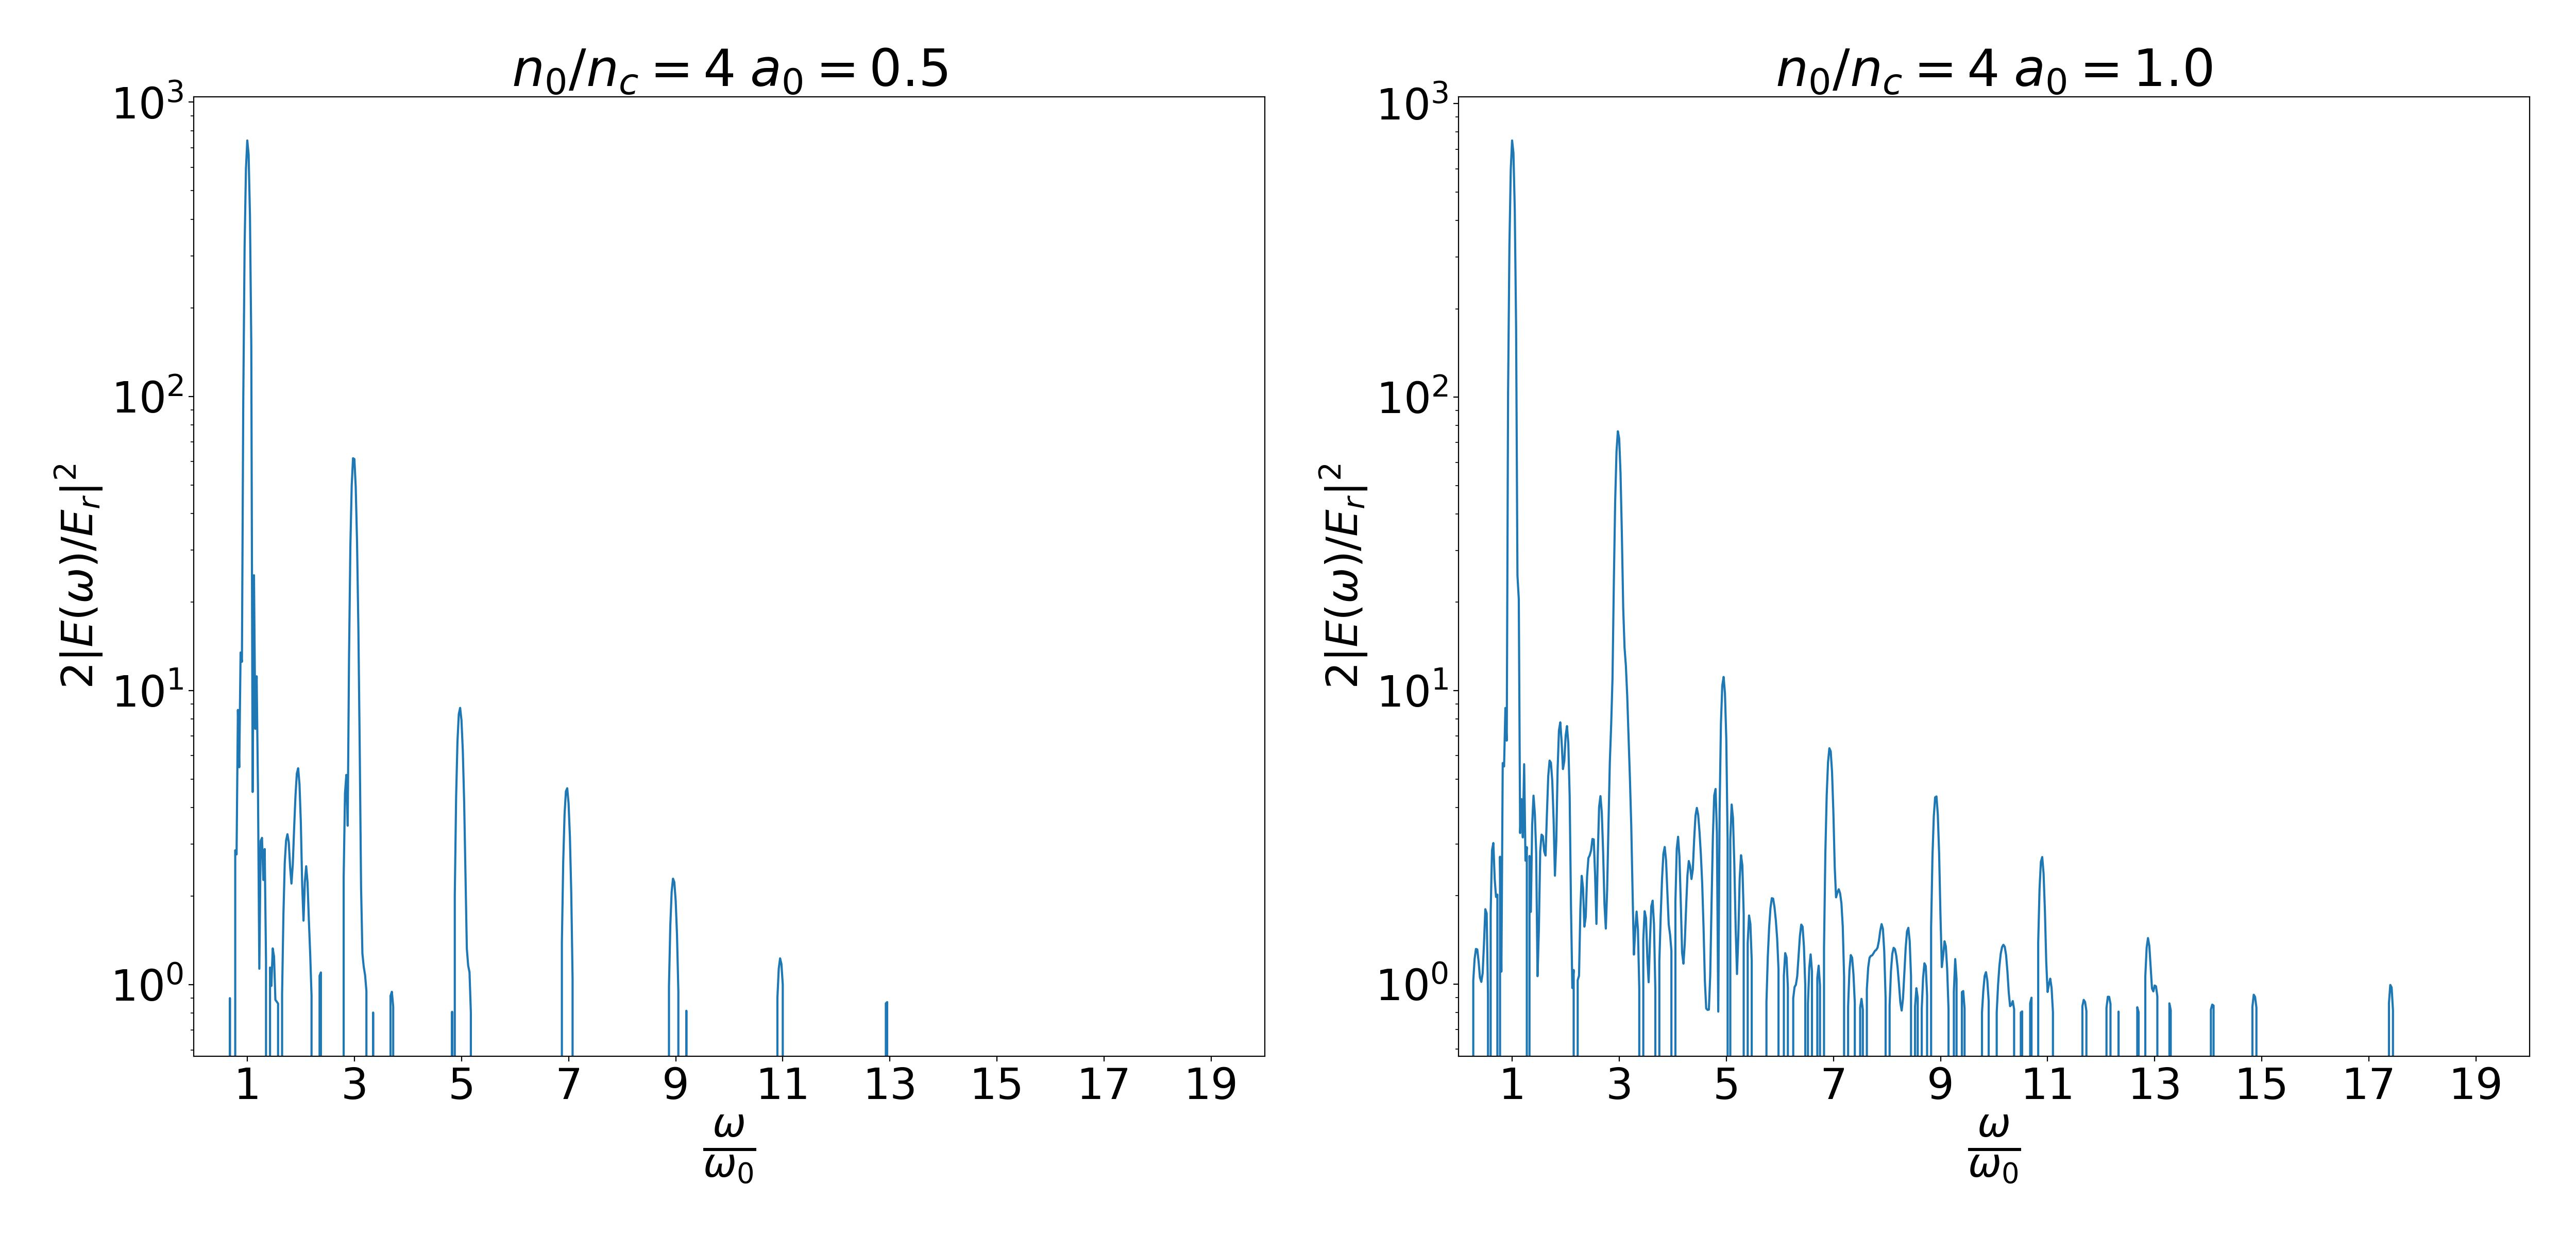
\includegraphics[width=0.85\textwidth]{intensity.jpg}
    \caption{Laser intensity and the harmonics generated.}
    \label{fig:intensity}
\end{figure}

\subsubsubsection{Effect of Laser Envelope}
The laser envelope does not seem to have any effect at all. See the Figure \ref{fig:env}.

\begin{figure}[H]
    \centering
    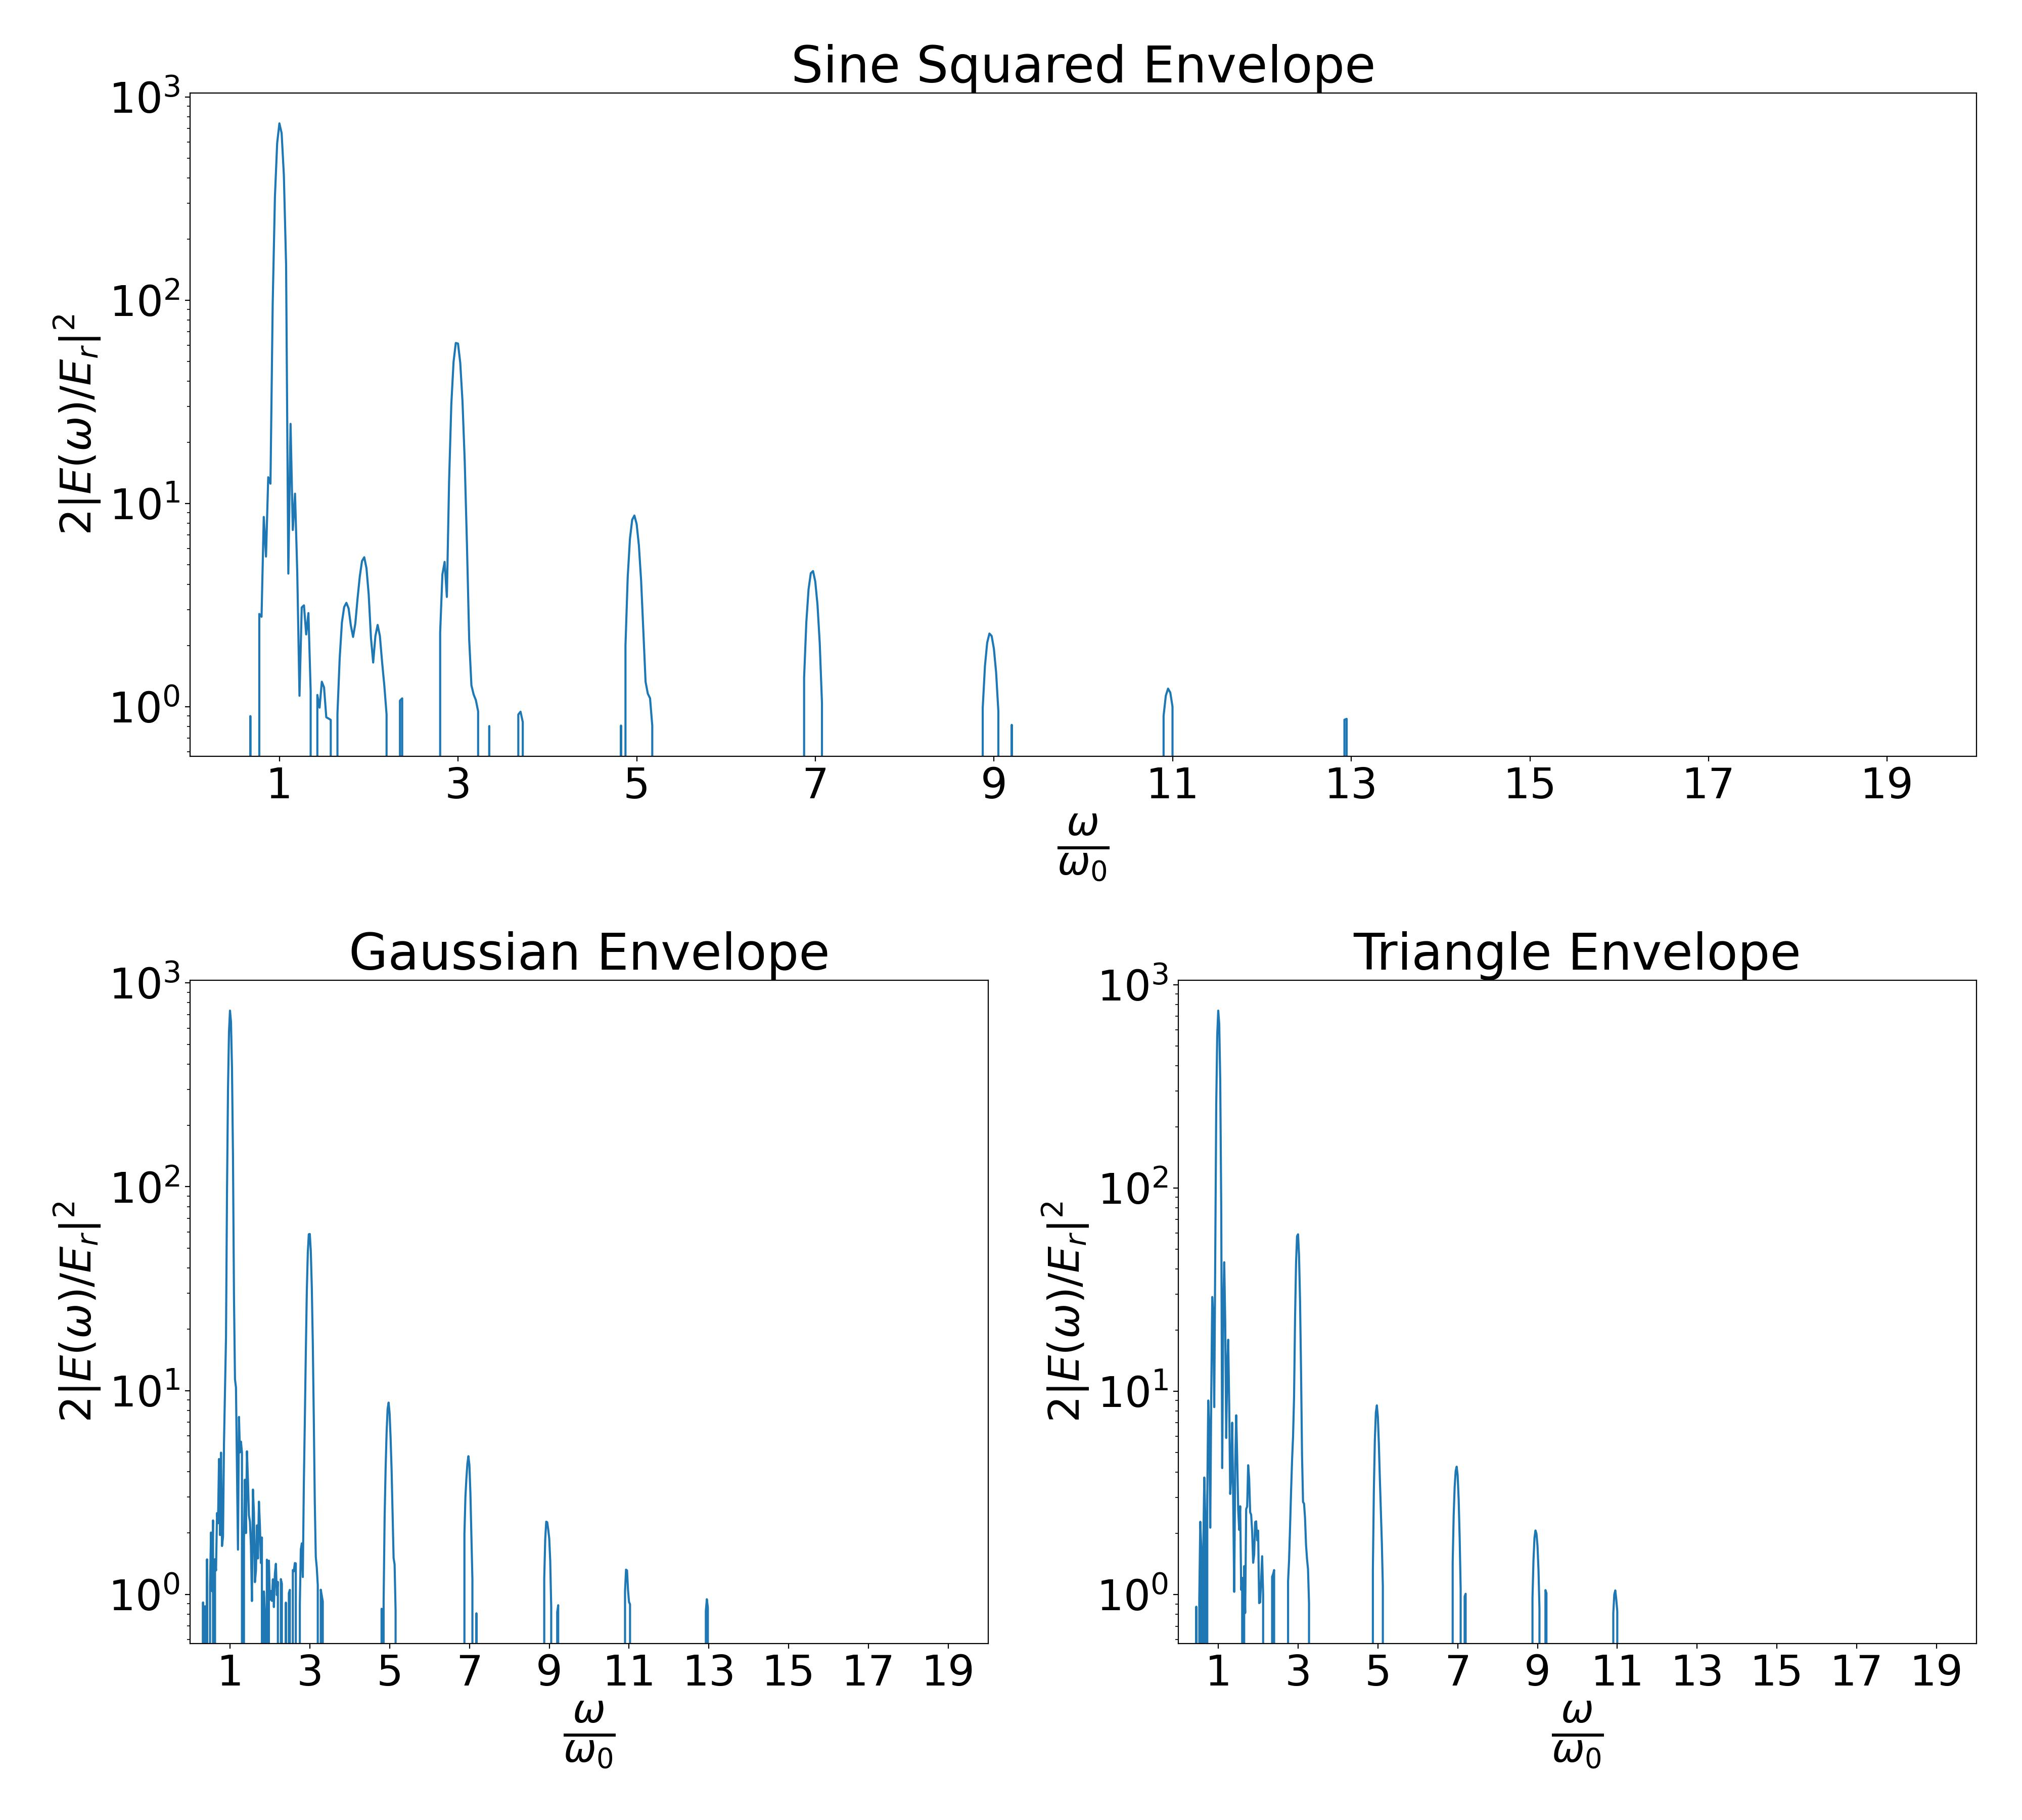
\includegraphics[width=0.85\textwidth]{env.jpg}
    \caption{Effect of the laser envelope on the harmonics generated. The plasma parameters are set to $a_0 = 0.5$ and $\frac{n_0}{n_c} = 4$.}
    \label{fig:env}
\end{figure}

\subsubsubsection{Super-Gaussian Envelope}

The SG envelope, given by equation \ref{eq:sg-env} has a different area for different $p$ and hence has different energy for the same given intensity. To mitigate this, the simulation is performed by multiplying the given intensity of the pulse such that the total energy of all the pulses is the same. This is done by taking a reference SG beam (we have used $p=2$), evaluating its area and then normalizing the intensities of other SG pulses by the ratio of this reference area and the area of the corresponding SG envelope. The spectrum of the HHG generated using laser pulse with SG envelopes with exponent 2, 4, 6, and 8 are shown in figure \ref{fig:sg} (a). It is observed that a small increase in the amplitude is followed by increasing exponent of the SG envelope. Next, we plot the amplitudes of different harmonics as a function of the exponent of SG function. It is clear from the Figure \ref{fig:sg} (b) that the amplitude of the harmonics increases as the exponent increases.

\begin{figure}[H]
    \centering
    \subfloat[\centering The spectrum of SG envelopes with exponent 2,6, and 20 are shown in a single plot. A small increase in the peak amplitude is observed with increasing exponent.]{{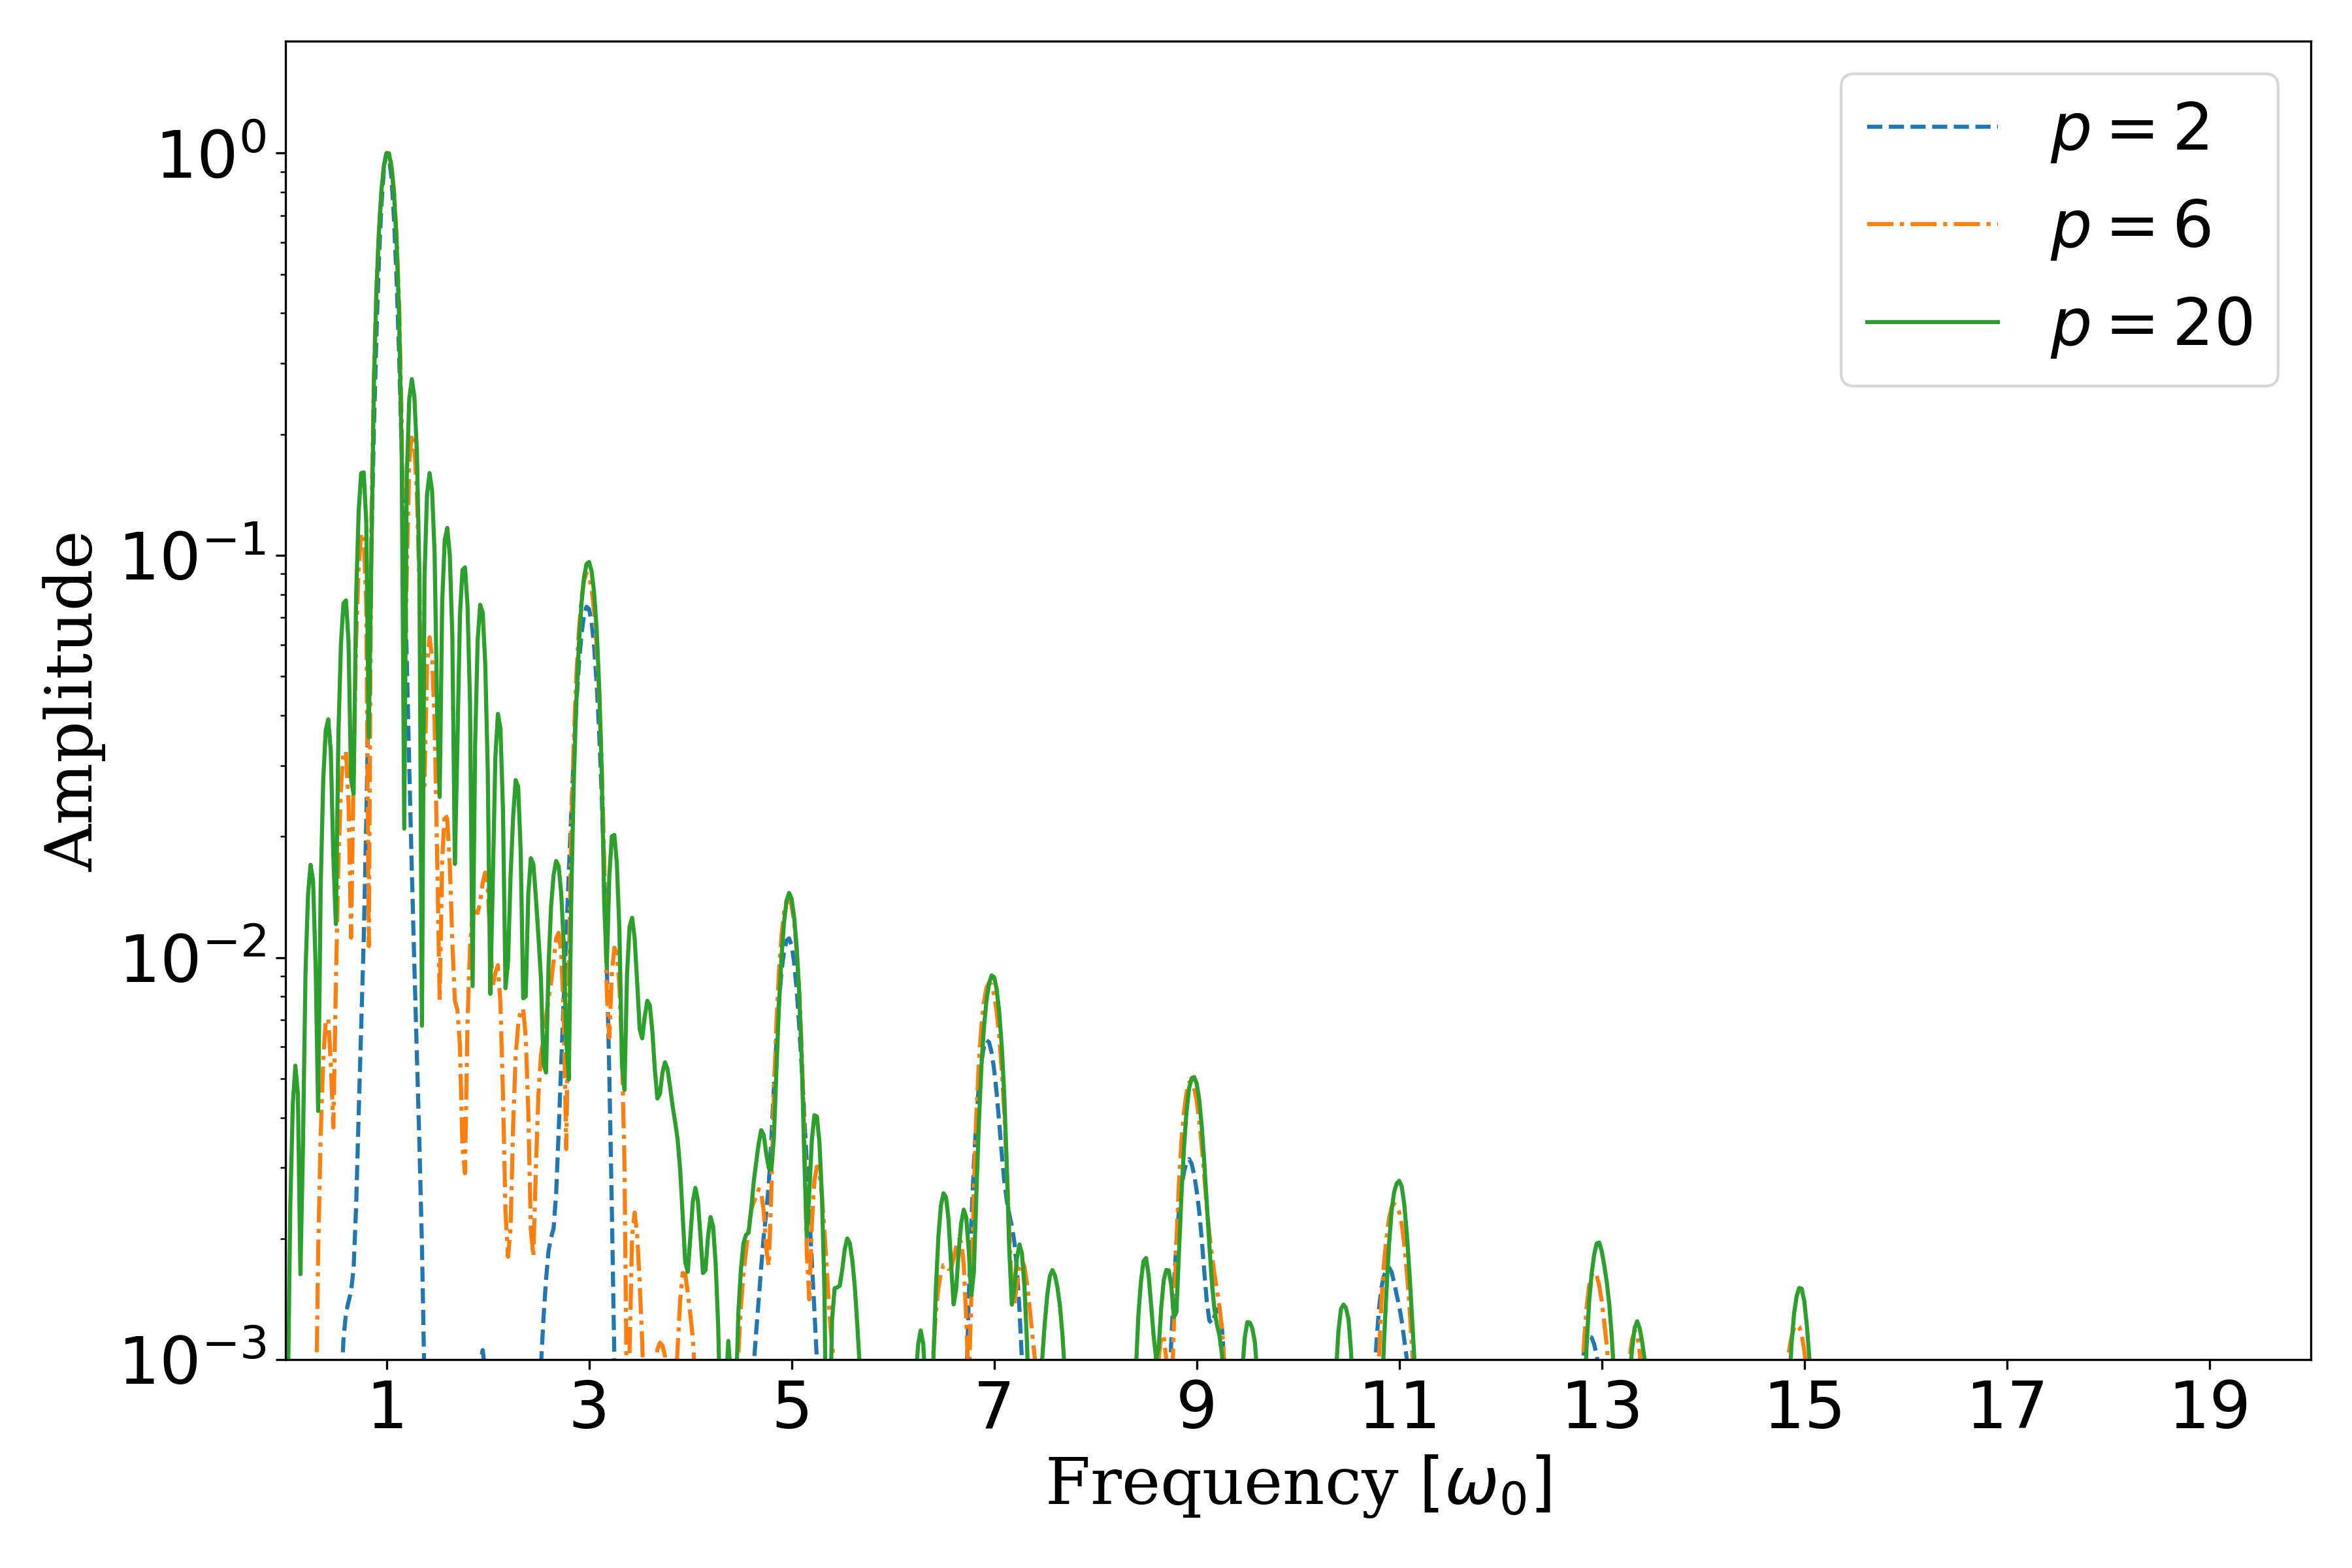
\includegraphics[width=0.47\textwidth]{SG_ffts_2-6-20.png}}}%
    \quad
    \subfloat[\centering The peak of different harmonics for different exponents is shown here. The amplitude increases as the exponent is increased.]{{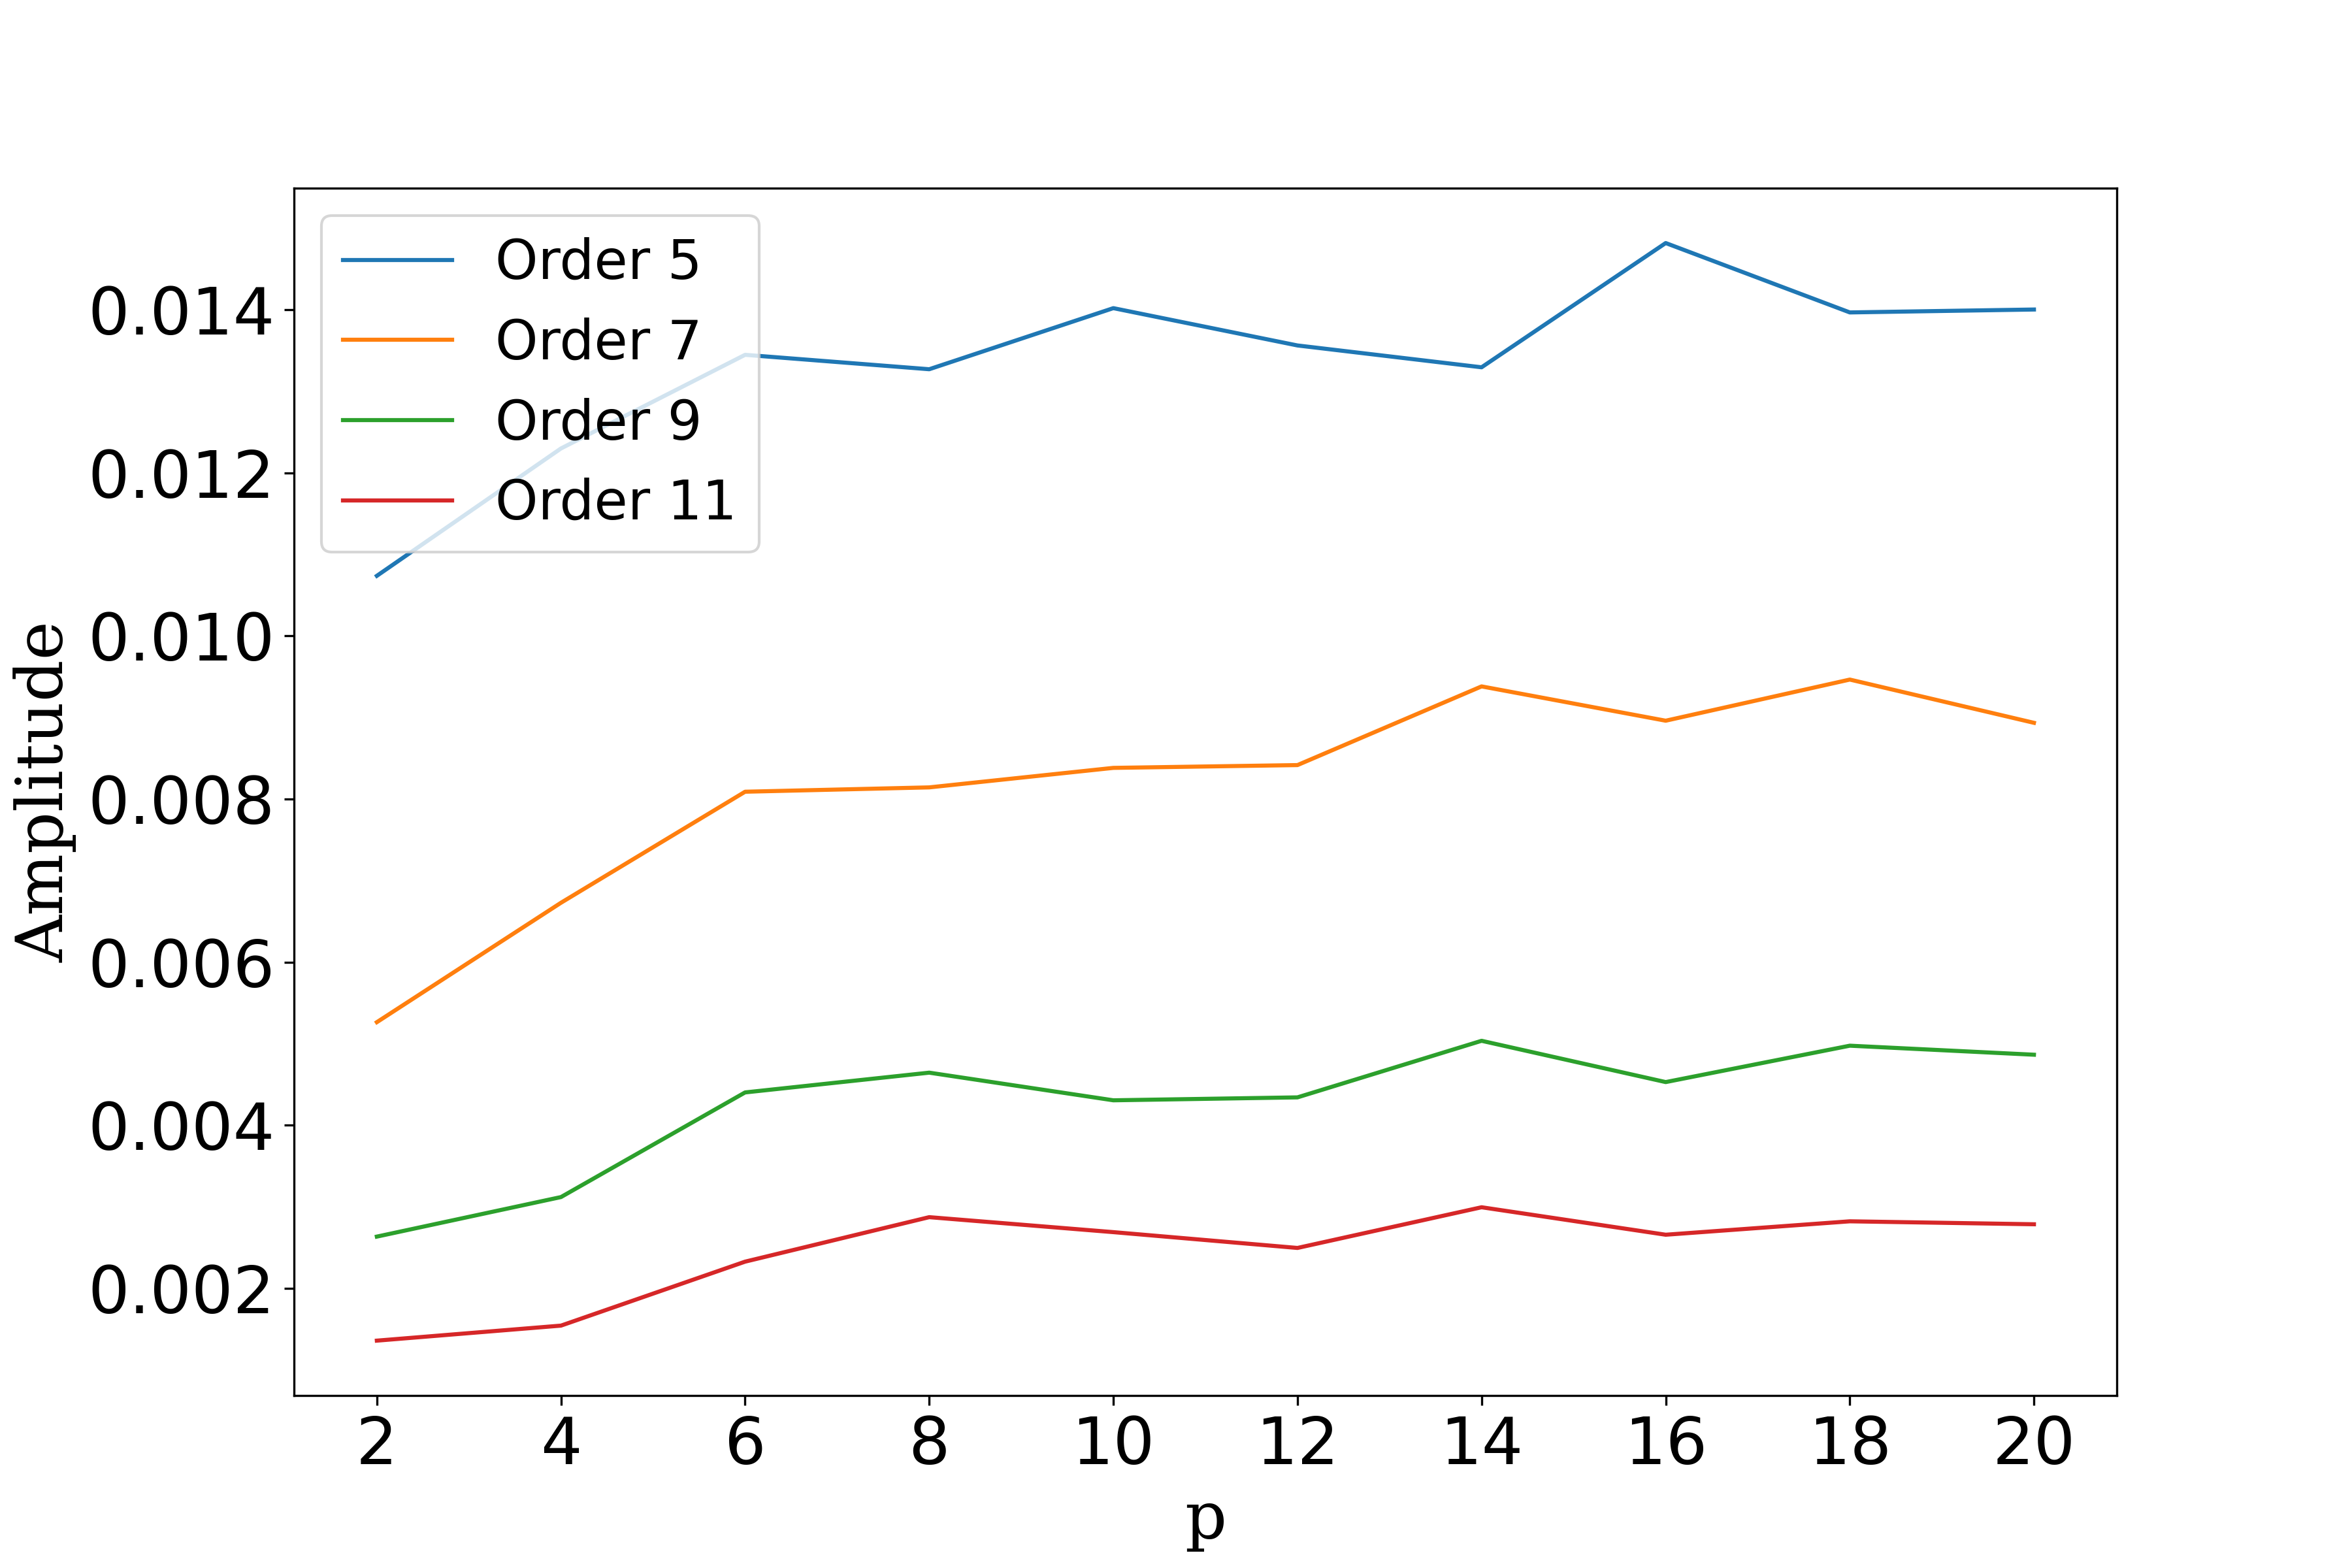
\includegraphics[width=0.47\textwidth]{SG_peak_amplitude.png}}}%
    \caption{SG Envelope. Parameters are $a_0 = 0.5$ and $\frac{n_0}{n_c} = 4$.}
    \label{fig:sg}%
\end{figure}

\begin{figure}[H]
    \centering
    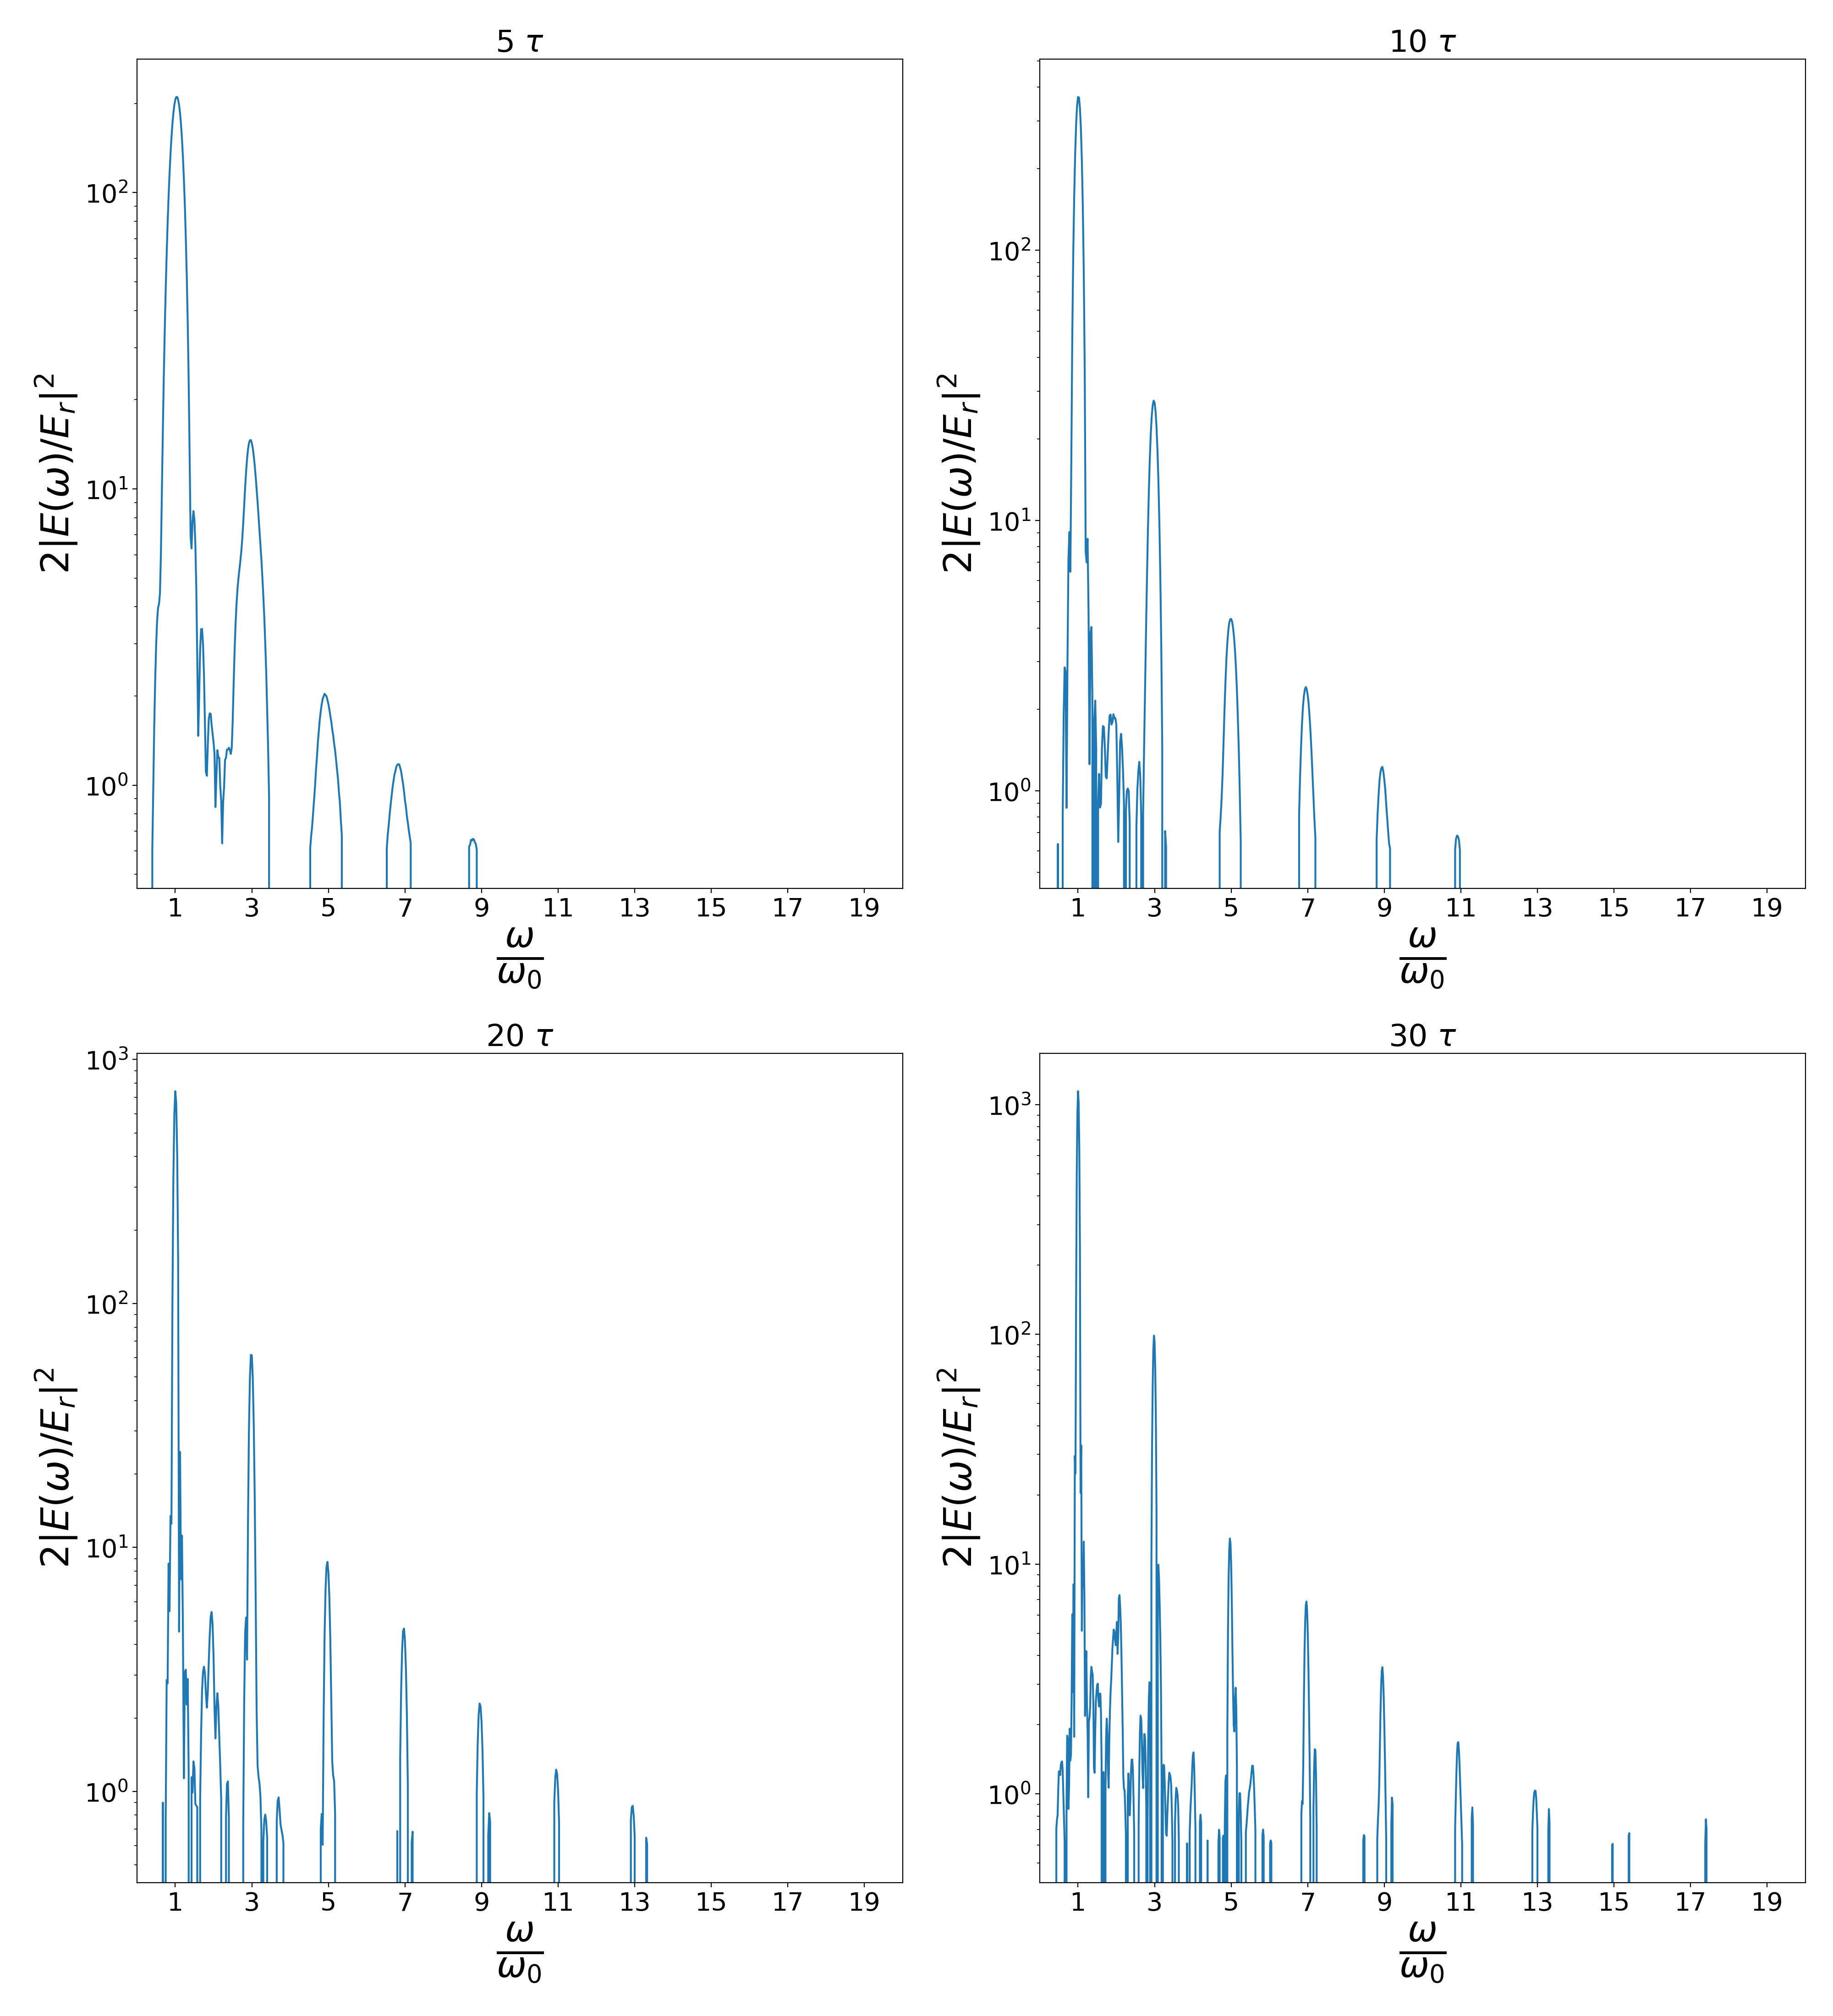
\includegraphics[width=0.80\textwidth, height=11cm]{pulse.jpg}
    \caption{Effect of the laser pulse duration on the harmonics generated. As pulse width increases, the amplitude of harmonics increases. The plasma parameters are set to $a_0 = 0.5$ and $\frac{n_0}{n_c} = 4$.}
    \label{fig:pulse}
\end{figure}

\subsubsubsection{Effect of Pulse Duration}

Increasing the pulse duration increases power within the pulse which then increases the number of harmonics generated. The harmonics also become more pronounced in amplitude.\cite{pulse-duration} The Figure \ref{fig:pulse} on shows the effect of the laser pulse duration on the harmonics generated.

\subsubsection{The Frequency of Plasma Oscillations}
The frequency of the plasma oscillations are determined in three different stages: before the laser interacts with the plasma (Figure \ref{fig:oscillation_1}), during the interaction (Figure \ref{fig:oscillation_2}) and after the interaction (Figure \ref{fig:oscillation_3}). We found out that the frequency of oscillations is even harmonic of the frequency of the incident laser pulse. Furthermore, electrons are oscillating only till they are interacting with the laser field. After the laser staops interacting with plasma, a frequency of about $2.6\omega_l$ is observed in the plasma oscillation. The oscillations are plotted along with the spectra. (See the Figure \ref{fig:oscillation_3}). In this simulation, we have used $a_0 = 0.5$ and $\frac{n_0}{n_c} = 7$.

\begin{figure}[H]
    \centering
    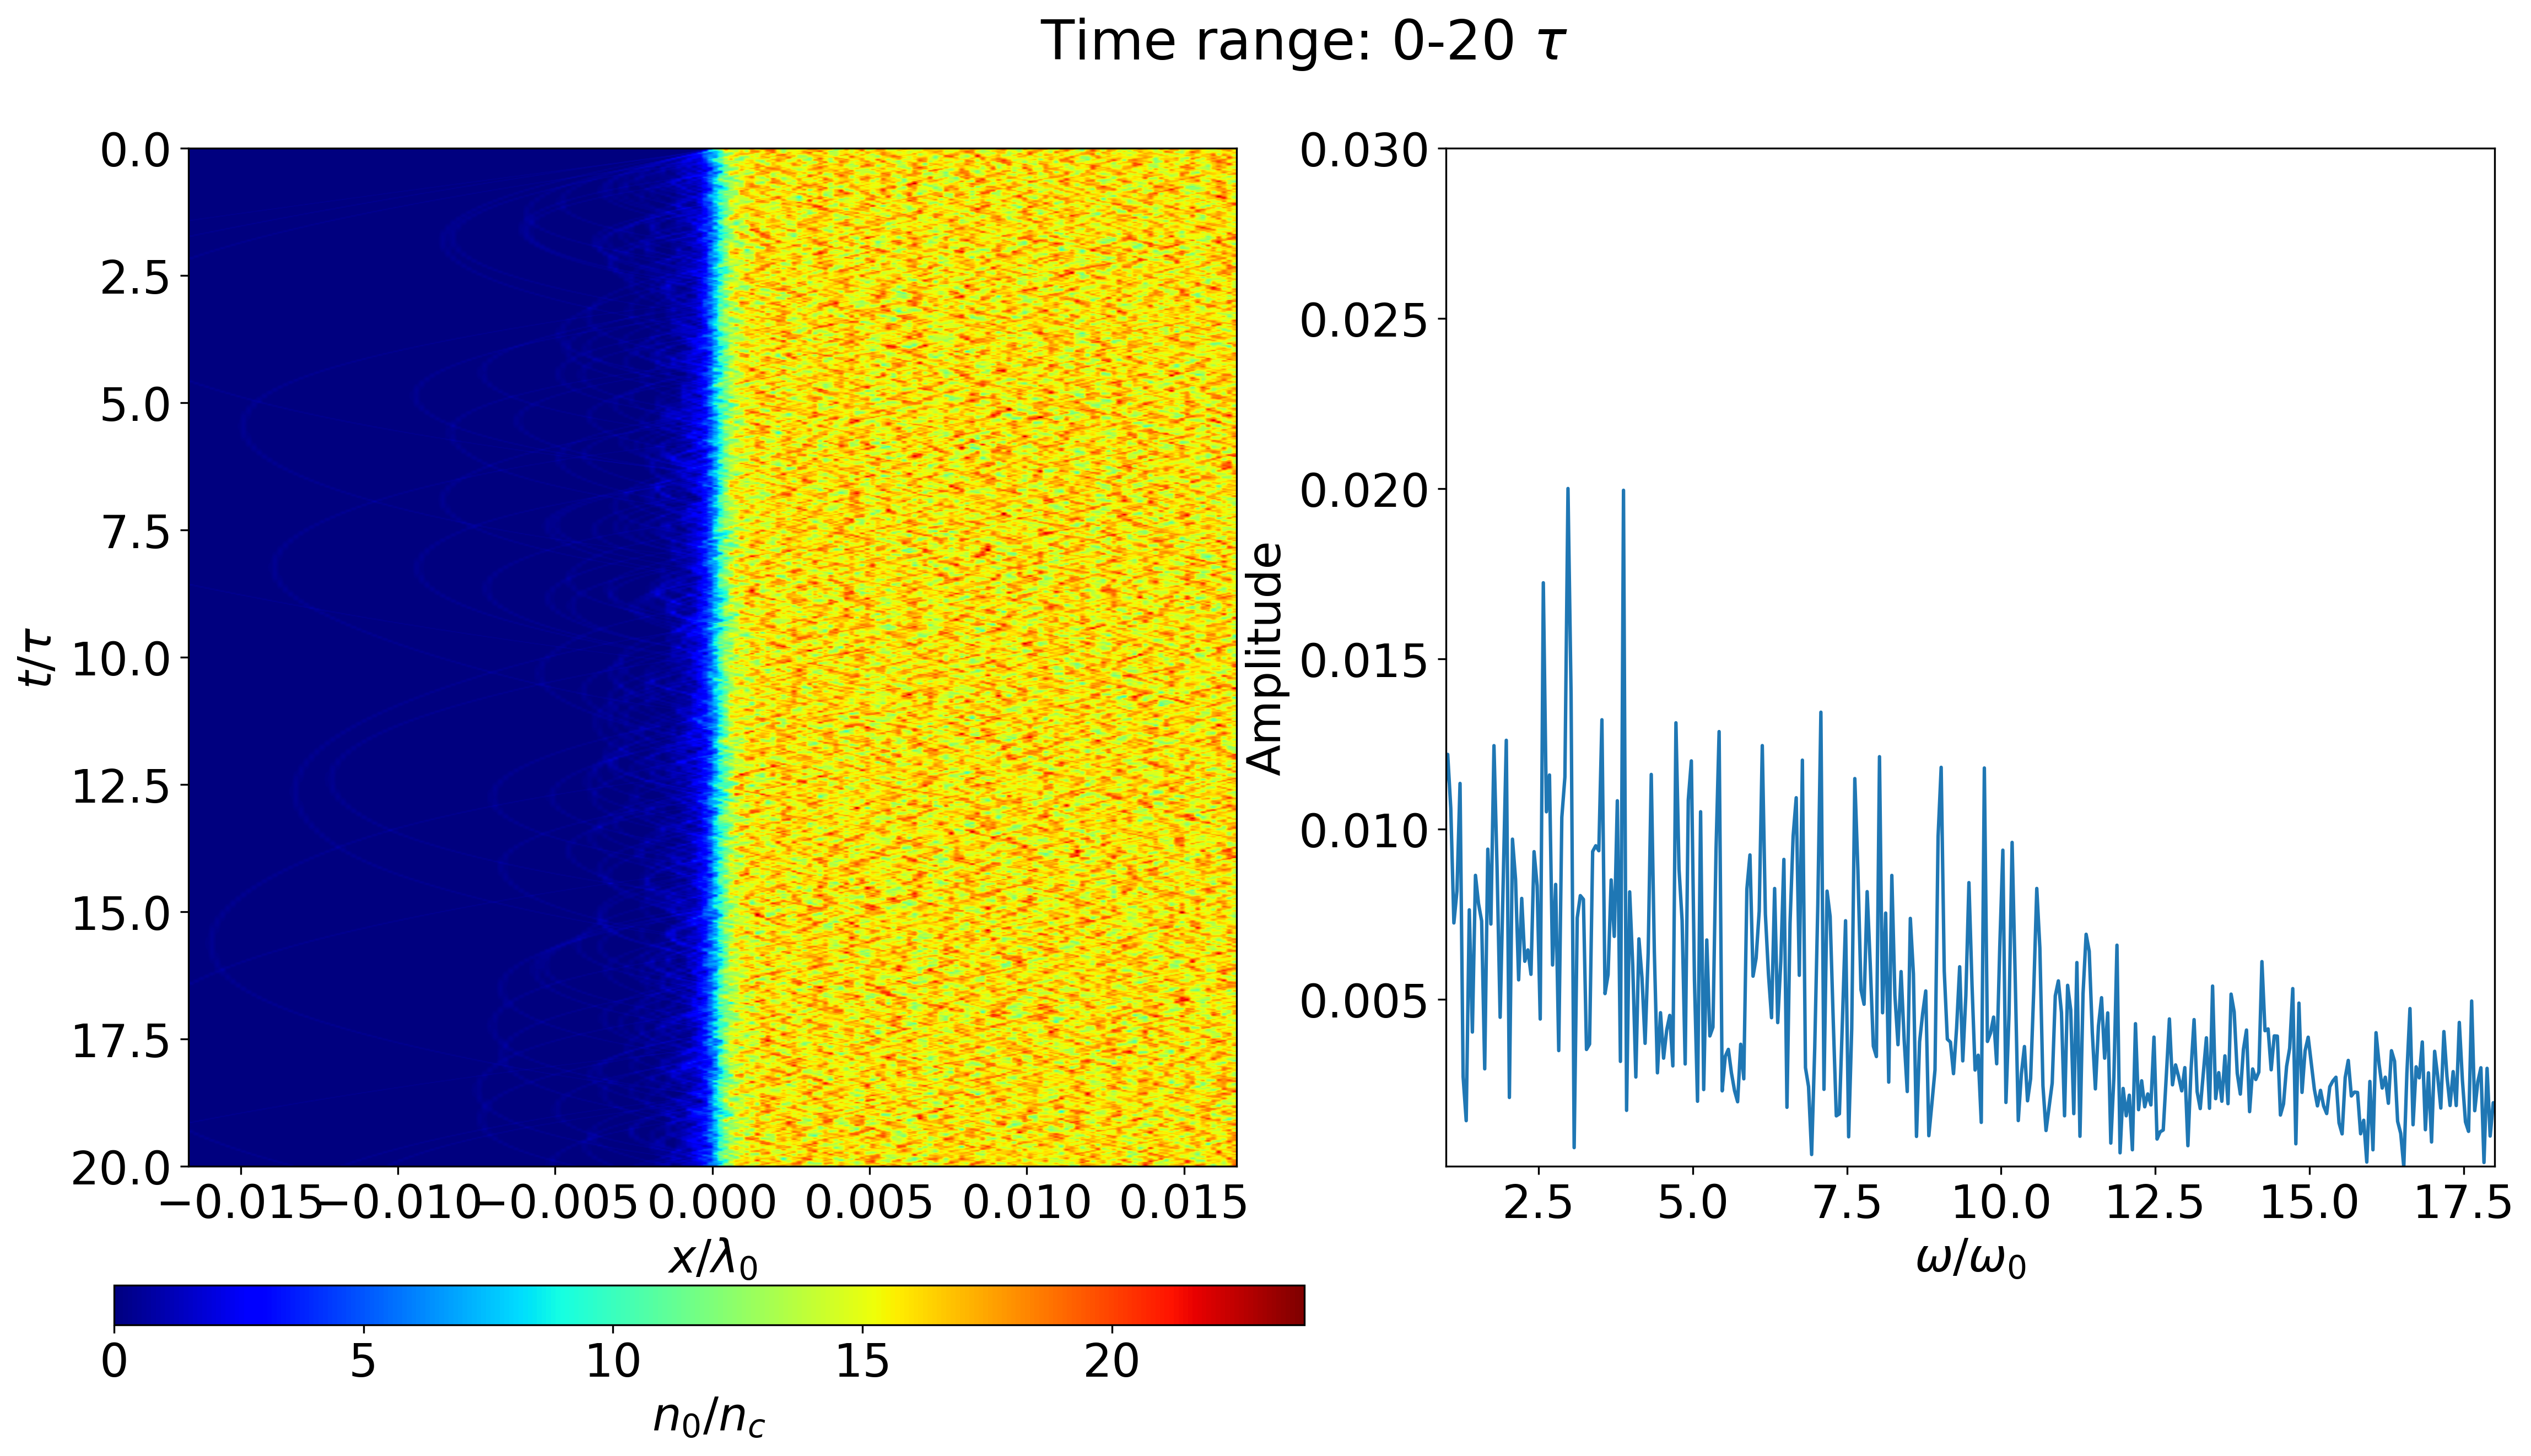
\includegraphics[width=0.75\textwidth]{oscillation_1.png}
    \caption{Frequency of electron oscillations before the laser interacts with plasma.}
    \label{fig:oscillation_1}
\end{figure}

\begin{figure}[h]
    \centering
    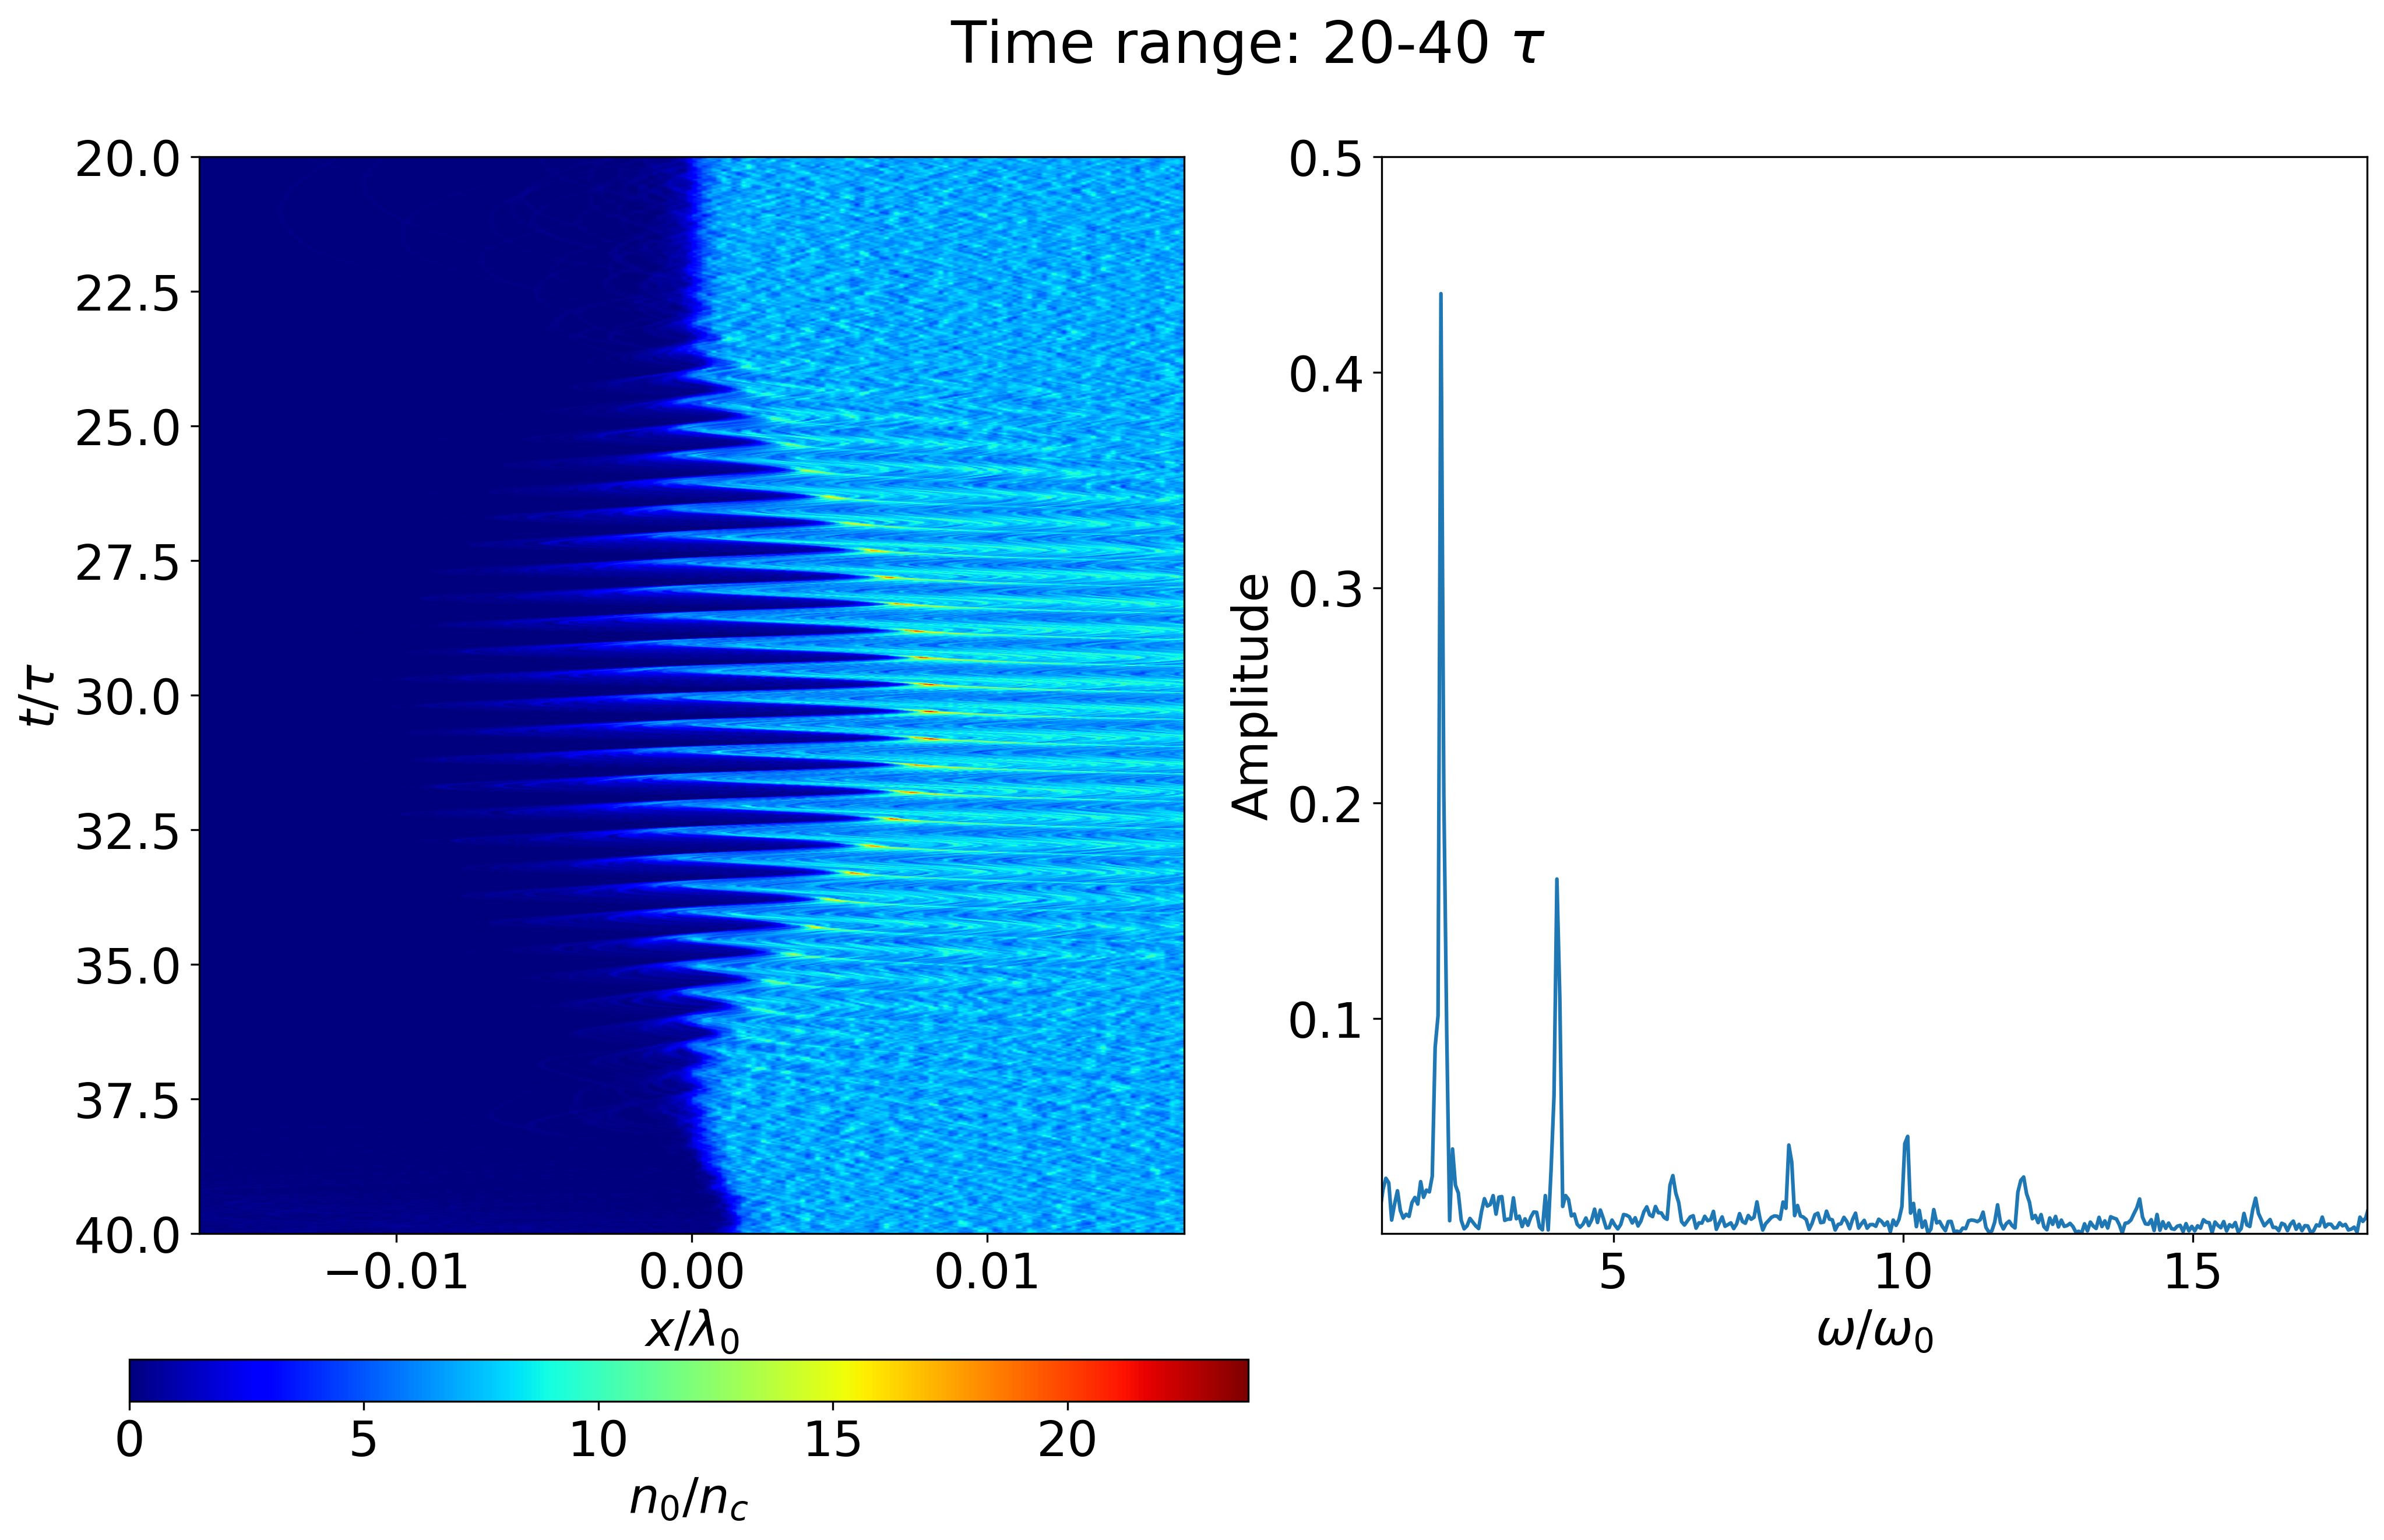
\includegraphics[width=0.75\textwidth]{oscillation_2.png}
    \caption{Frequency of electron oscillations during the laser is interacting with plasma.}
    \label{fig:oscillation_2}
\end{figure}

\begin{figure}[h]
    \centering
    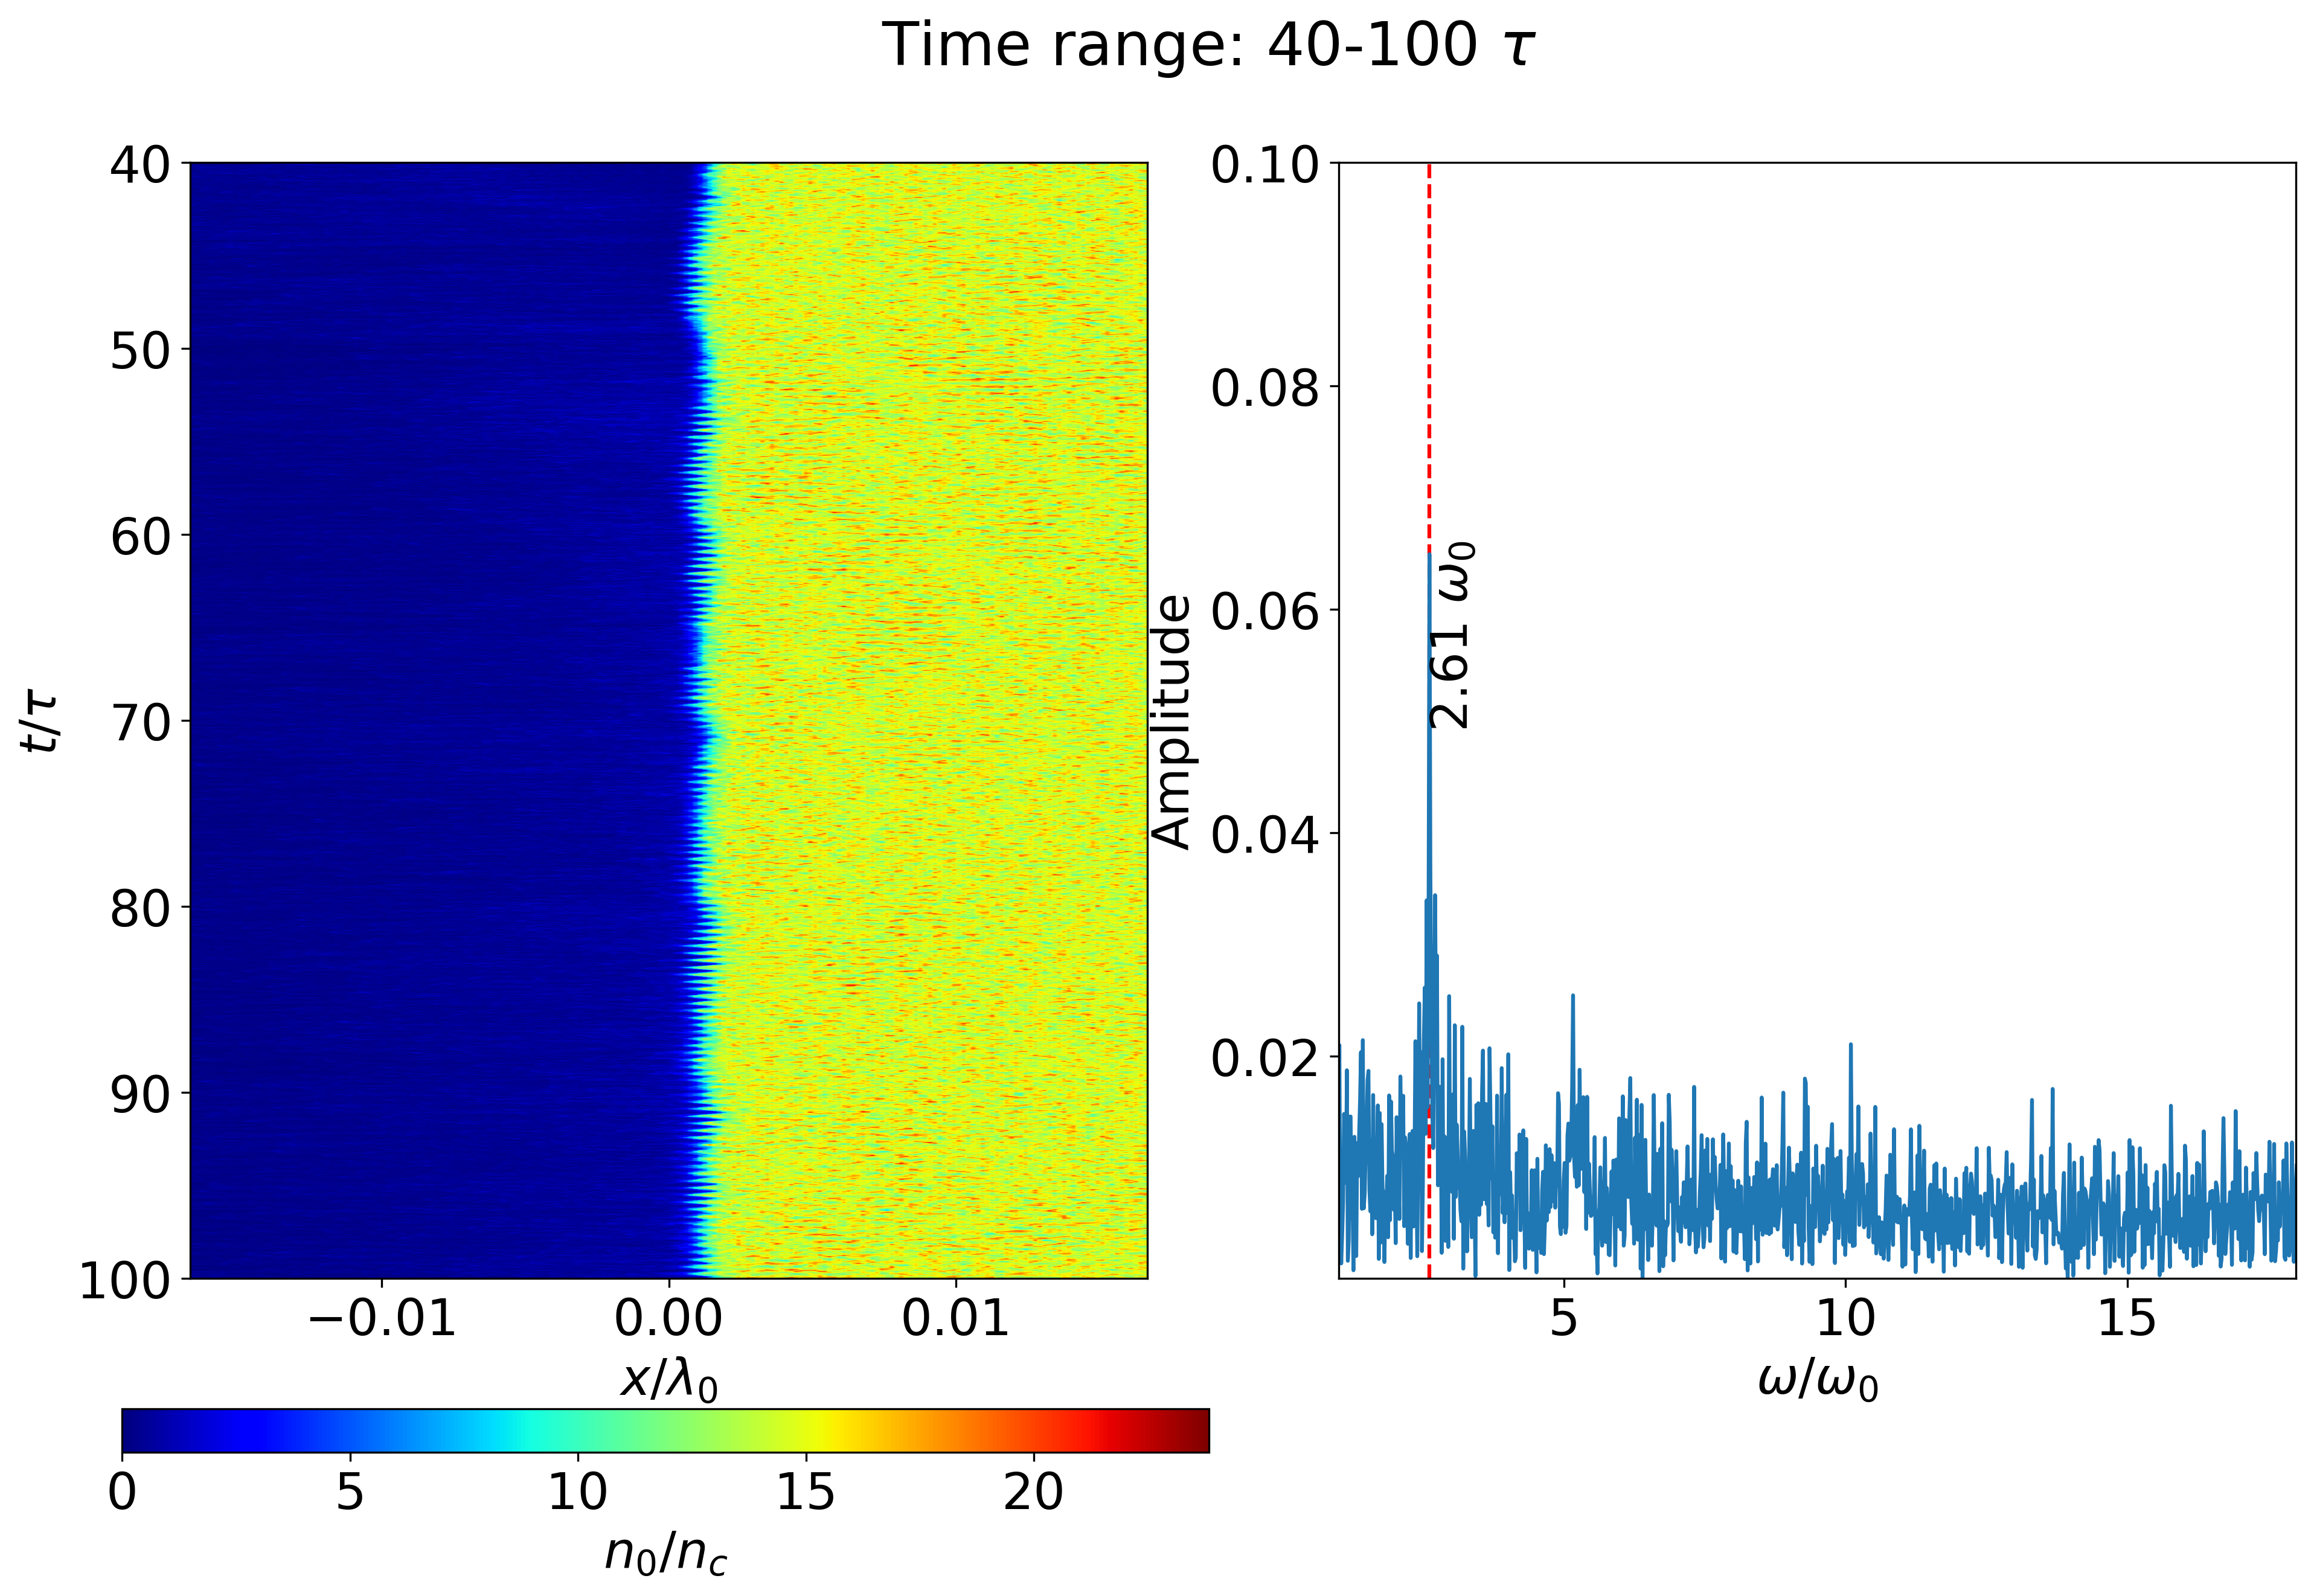
\includegraphics[width=0.75\textwidth]{oscillation_3.png}
    \caption{Frequency of electron oscillations after the laser interacts with plasma.}
    \label{fig:oscillation_3}
\end{figure}

\subsection{Oblique Incidence}

\subsubsection{p-Polarization}
Figure \ref{fig:p-fft} shows the spectrum of HHG in the L-frame, when p-polarized light is incident on the plasma. As discussed in section \ref{section:selection} (see the table \ref{tab:selection-rule}), the spectrum is made up of even and odd p-polarized harmonics. There are no s-polarized harmonics.

\begin{figure}[H]
    \centering
    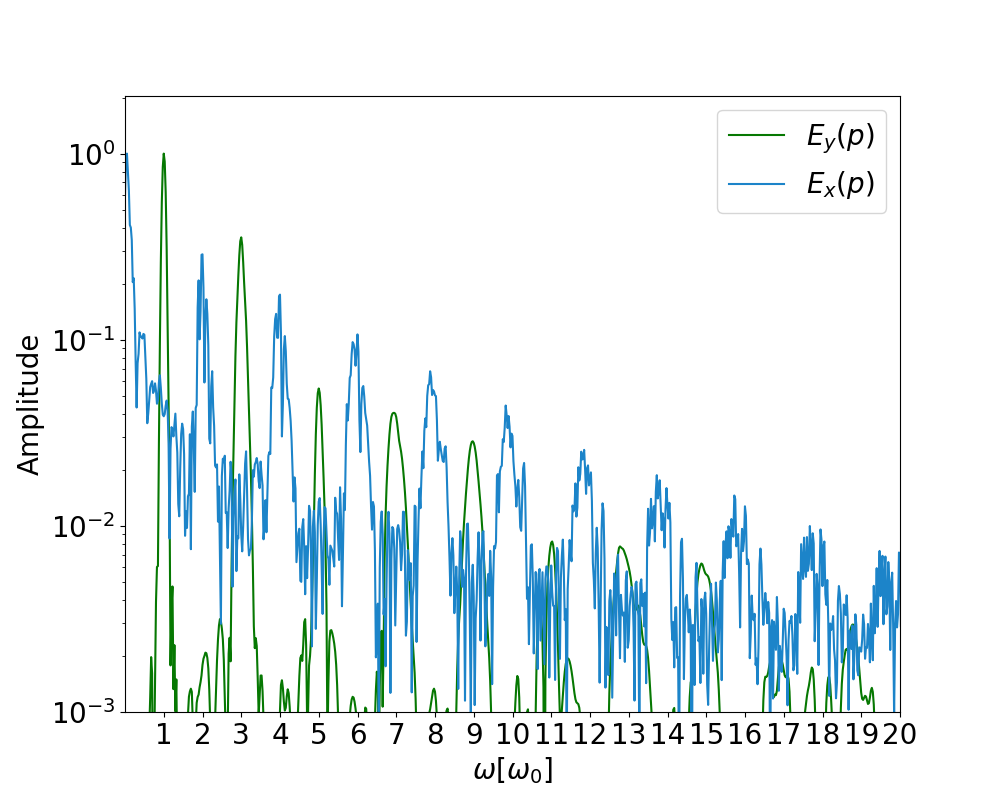
\includegraphics[width=0.8\textwidth]{p_fft.png}
    \caption{The spectrum of HHG for p-polarized light. Simulation parameters are $\alpha = \pi/4$, the density is $n_0 = 7n_c$ and $a_0 = 4$. We see that both odd and even harmonics generated are p-polarized.}
    \label{fig:p-fft}
\end{figure}


\subsubsection{s-Polarization}
The L-frame spectrum of HHG is depicted in diagram \ref{fig:s-fft}, with plasma being exposed to s-polarized light. As explained in section \ref{section:selection} (see the table \ref{tab:selection-rule}), the spectrum comprises odd s-polarized harmonics and even p-polarized harmonics.
\begin{figure}[h]
    \centering
    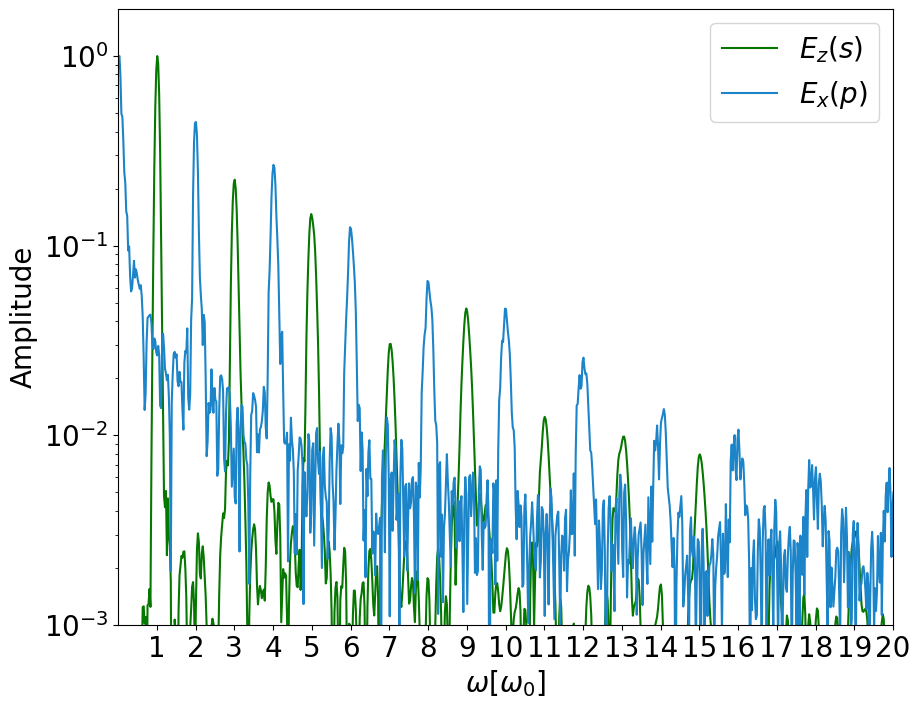
\includegraphics[width=0.85\textwidth]{s_fft.png}
    \caption{The spectrum of HHG for s-polarized light. Simulation parameters are $\alpha = \pi/4$, the density is $n_0 = 7n_c$ and $a_0 = 4$. Here s-polarized odd and p-polarized even harmonics are generated.}
    \label{fig:s-fft}
\end{figure}
